%%%%% START PREAMBLE HEADER %%%%%

%%% START REQUIRED PACKAGES %%%

\documentclass{article}
\usepackage{xcolor} 
\usepackage[a4paper, total={7.25in, 9.5in}]{geometry} 
\usepackage{multirow}
\usepackage{lipsum}
\usepackage{hyperref}
\usepackage{listings}
\usepackage{graphicx}
\usepackage[export]{adjustbox}
%\usepackage[superscript,biblabel]{cite}
\usepackage{amsmath}
\usepackage[utf8]{inputenc}
\hypersetup{colorlinks=true,linkcolor=blue,filecolor=magenta,urlcolor=cyan,citecolor=blue}

%%% END REQUIRED PACKAGES %%%                


%%% START NEW COMMANDS new (shortcut) %%%

% This is a paragraph with normal font
\newcommand{\np}[1]{\paragraph*{\normalfont{#1}}}
% This is a text with a color
\newcommand{\ct}[2]{\textcolor{#1}{#2}}
% This is a bold text 
\newcommand{\bt}[1]{\textbf{#1}}
% This is an italic text 
\newcommand{\et}[1]{\emph{#1}}
% This is an underline text 
\newcommand{\ut}[1]{\underline{#1}}
% This is a newline shortcut
\newcommand{\n}{\\}
% This is a numbered equation with break line shortcut
\newcommand{\necbreak}[1]{\begin{equation}\begin{aligned}#1\end{aligned}\end{equation}}
% This is a equation with break line shortcut
\newcommand{\ecbreak}[1]{\begin{center}\begin{gather*}#1\end{gather*}\end{center}}
% This is a numbered equation with break line shortcut
\newcommand{\nec}[1]{\begin{equation}#1\end{equation}}
% This is an equation shortcut
\newcommand{\ec}[1]{\begin{center} $#1$ \end{center}}
% Table title with bold text and correct space%
\newcommand{\titleTable}[2]{\np{\bt{Table #1} #2}}% Graph title with bold text and correct space%
\newcommand{\titleGraph}[2]{\np{\bt{Graph #1} #2}}
% Table body with border %
\newcommand{\bodyTable}[2]{\begin{center} \begin{tabular}{|#1|} \hline #2 \hline \end{tabular} \end{center} }
%%% END NEW COMMANDS (shortcuts) %%%


%%% START TITLE SETTINGS %%%
\title{Fisicoquímica de sistemas moleculares organizados \n Tarea 1 Serie de problemas }
\author{Pérez Alvarado Luis Raymundo, Facultad de Química, UNAM}
\date{06/11/2020}
%%% END TITLE SETTINGS %%%

%%%%% END PREAMBLE HEADER %%%%%

%%%%%%%%%%%%%%%% START DOCUMENT %%%%%%%%%%%%%%%%
\begin{document}

    \maketitle

    \np{\bt{1)} ¿Será necesario una mayor cantidad de energía si se desea colocar un ión potasio en el interior de la proteína?}

    \np{DATOS: radio del $Na^+=1.94$ \AA, radio del $Cl^-+=1.21$ y $D_{prot}=3.5D_0$ \AA }

    \np{Primero se procede a calcular el $\Delta E$ del $Na+$ y el $Cl^-$ en medio acuoso y dentro de la proteína, se emplea la ecuacion \ref{equation:1} para calcular la energía necesaria para tener un ión dentro de una proteína.}

    \nec{\label{equation:1} E_s = \frac{q^2}{2D_{ion}R_{Stokes}}}

    \np{Se tienen constantea los siguientes datos $q=1.6022x10^{-19}C$, $D_{H_2O}=78.5D_0$ y $D_0=4\pi 8.885x10^{-12}C^2J^{-1}m^{-1}$}

    \np{Se convierten las unidades de \AA~a metros usando el factor de conversión $(\frac{1x10^{-10}~m}{1~\text{\AA}})$ }

    \np{Se calcula la auto energía de cada ion en agua empleando la ecuación \eqref{equation:1}.}

    \ec{
        E_{Na^{+}_{H_2O}}=\frac{(1.6022x10^{-19}C)^2}{2(78.5)(4\pi 8.885x10^{-12}C^2J^{-1}m^{-1})(1.94x10^{-10}m)}(\frac{6.022x10^{23}}{mol})(\frac{1kJ}{1000J})=5.249 kJ/mol
    }

    \ec{
        E_{Cl^{-}_{H_2O}}=\frac{(1.6022x10^{-19}C)^2}{2(78.5)(4\pi 8.885x10^{-12}C^2J^{-1}m^{-1})(1.21x10^{-10}m)}(\frac{6.022x10^{23}}{mol})(\frac{1kJ}{1000J})=4.545 kJ/mol
    }

    \np{Se calcula la auto energía de cada ion dentro de la proteina empleando la ecuación \eqref{equation:1}.}

    \ec{
        E_{Na^{+}_{prot}}=\frac{(1.6022x10^{-19}C)^2}{2(3.5)(4\pi 8.885x10^{-12}C^2J^{-1}m^{-1})(1.94x10^{-10}m)}(\frac{6.022x10^{23}}{mol})(\frac{1kJ}{1000J})=117.736 kJ/mol
    }

    \ec{
        E_{Cl^{-}_{prot}}=\frac{(1.6022x10^{-19}C)^2}{2(3.5)(4\pi 8.885x10^{-12}C^2J^{-1}m^{-1})(1.21x10^{-10}m)}(\frac{6.022x10^{23}}{mol})(\frac{1kJ}{1000J})=101.957 kJ/mol
    }

    \np{\bt{Si es necesario más energía para tener un ion potasion dentro de la proteinas, esto se observa al comparar la energía de auto energia del ion en agua y dentro de la proteína.}}
    
    %PROBLEMA 2%
    
    \np{\bt{2)} ¿Cual sería el operador de simetría especular $\hat{i}$ para el plano $y-z$ y $x-y$?}

    \np{El siguiente sistema de ecuaciones se emplea para describir las coordenadas de un sistema cartesiano después de aplicar un operador $\hat{X}$.}

    \necbreak{\label{equation:2}
        & a_1x+b_1y+c_1z=x'\\
        & a_2x+b_2y+c_2z=y'\\
        & a_3x+b_3y+c_3z=z'
    }

    \np{El determinante para un operador $\hat{X}$ para un sistema de coordenadas cartesianas lo describimos de la siguiente forma.}

    \nec{\label{equation:3}
        \hat{X}= 
        \begin{vmatrix}
            a_1 &b_1& c_1\\
            a_2&b_2&c_2\\
            a_3&b_3 &c_3\\
        \end{vmatrix}
        \text{x}
        \begin{vmatrix}
            x\\
            y\\
            z\\
        \end{vmatrix}
        =
        \begin{vmatrix}
            x'\\
            y'\\
            z'\\
        \end{vmatrix}
    }

    \np{Considerando el plano y-z se obtiene que los valores de los coeficientes del determinante general \eqref{equation:2} y en el sistema de ecuacion \eqref{equation:3} se obtiene.}

    \ec{
        \begin{vmatrix}
            -1&0&0\\
            0&1&0\\
            0&0&1\\
        \end{vmatrix}
        \text{x}
        \begin{vmatrix}
            x\\
            y\\
            z\\
        \end{vmatrix}
        =
        \begin{vmatrix}
            -x\\
            y\\
            z\\
        \end{vmatrix}
    }

    \ecbreak{
        -1(x)+0(y)+0(z)=-x\\
        0(x)+1(y)+0(z)=y\\
        0(x)+0(y)+1(z)=z
    }

    \np{Por lo que operador especular del plano $y-z$ es \bt{$\hat{i}_{y-z}(x,y,z)=(x',y',z')=(-x,y,z)$}}

    \np{Considerando el plano x-y se obtienen el siguiente determinante y se sustituyen los coeficientes en el sistema de ecuaciones.}

    \ec{
        \begin{vmatrix}
            1&0&0\\
            0&1&0\\
            0&0&-1\\
        \end{vmatrix}
        \text{x}
        \begin{vmatrix}
            x\\
            y\\
            z\\
        \end{vmatrix}
        =
        \begin{vmatrix}
            x\\
            y\\
            -z\\
        \end{vmatrix}
    }

    \ecbreak{
        1(x)+0(y)+0(z)=x\\
        0(x)+1(y)+0(z)=y\\
        0(x)+0(y)-1(z)=-z
    }

    \np{Por lo que operador especular del plano $x-y$ es \bt{$\hat{i}_{x-y}(x,y,z)=(x',y',z')=(x,y,-z)$}}

    %PROBLEMA 3%
    
    \np{\bt{3)} ¿Cuál sería el operador de simetría helicoidal si se toma al eje $y$ como el eje de la hélice?}

    \np{\bt{3)} Primero se calcula el operador de simetria rotacional $\hat{C}$, se contruye el determinante y en base al plano $x-z$ considerando un ángulo de $180^o$ al motivo se obtiene lo siguiente.}  

    \ec{\hat{C}_{x-z}= 
        \begin{vmatrix}
            -1 &0& 0\\
            0&1&0\\
            0& 0 &-1\\
        \end{vmatrix}
        \text{x}
        \begin{vmatrix}
            x\\
            y\\
            z\\
        \end{vmatrix}
        =
        \begin{vmatrix}
            -x\\
            y\\
            -z\\
        \end{vmatrix}
    }

    \np{Se expresan los coeficientes en términos de $\theta$ y se agrega el desplazamiento sobre el eje $y$ con el operador translacional $T$ y se obtiene lo siguiente.}

    \ec{
        \hat{C}_{x-z}+T_y=
        \begin{vmatrix}
            cos(\theta)&0& -sen(\theta)\\
            0&1&0\\
            sen(\theta)& 0 &cos(\theta)\\
        \end{vmatrix}
        \text{x}
        \begin{vmatrix}
            x\\
            y\\
            z\\
        \end{vmatrix}
        +
        \begin{vmatrix}
            0\\
            h\\
            0\\
        \end{vmatrix}
        =
        \begin{vmatrix}
            -x\\
            y+h\\
            -z\\
        \end{vmatrix}
    }

    \np{Por lo que operador helicoidal tomando al eje $y$ como eje de la hélice es \bt{$\hat{C}_{x-y}(x,y,z)+T_y=(x',y',z')=(-x,y+h,-z)$}}

    %PROBLEMA 4%
    
    \np{\bt{4)} ¿En cuál de las dos proteínas será más fácil colocar una carga en su interior?}

    \np{Se espera que sea más fácil colocar una carga dentro de la proteína mutada debido a que podran tener más conformaciones y se verá reflejado como un aumento en la entropía, por lo que se espera que la autoenergía sea menor que en la proteína natural.}

    %PROBLEMA 5%
    
    \np{\bt{5)} Dibuje un dipéptido en una hoja de papel (No importa que residuos de amino  ́acido emplee). ¿Cuántos tipos distintos de enlace covalente encuentra en el dipéptido? Indique en su dibujo los enlaces alrededor de
    los cuales es posible tener giros y cuales giros son descritos por los ángulos 
    $\phi$ y $\psi$. ¿Existen enlaces que no puedan girar? ¿Por qué?}

    % START FIGURE %
    \begin{figure}[h]
        \centering
        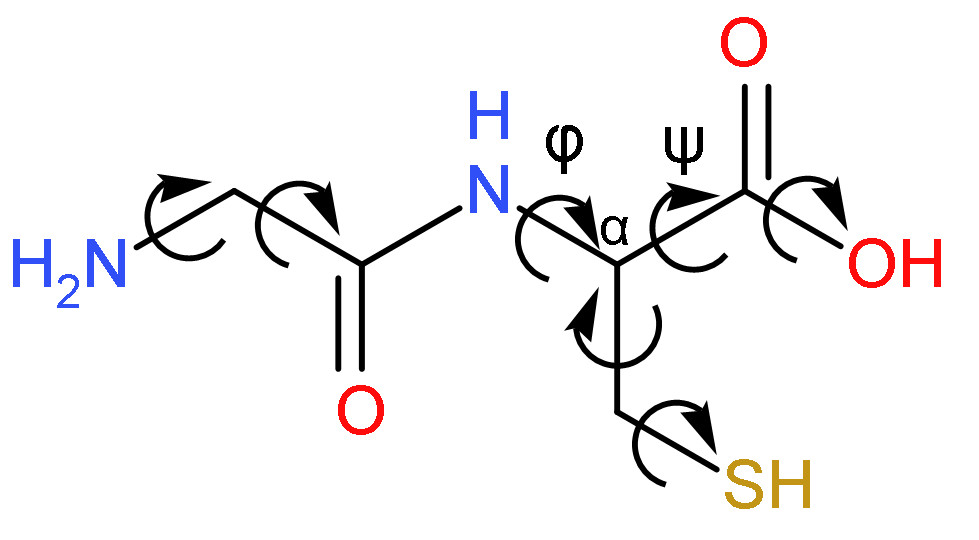
\includegraphics[scale=0.5]{GlyCys.jpg}
        \caption{Dipéptido Gly-Cys.}
    \end{figure}
    % END FIGURE %

    \np{Hay dos tipos de enlaces presentes, enlaces sencillos y dobles, dentro del sencillo se hace distinción del enlace peptídico.}

    \np{Los enlaces C=O no son capaces de rotar libremente que los dobles enlaces son rígidos, por lo que no tiene capacidad de rotar, los enlaces sencillos son capaces de rotar libremente(esto se ilusta con flechas negras) y en el enlace peptídico, este presenta un caracter de doble enlace, ya que la densidad electrónica esta entre se reparte entre el átomo de N y O, por lo que no presenta rotación.}

    %PROBLEMA 6%
    
    \np{\bt{6)} Identifique a los ángulos de torsión $\phi$ y $\psi$. Mueva los ángulos de torsión y mida distancias atómicas entre los átomos separados por más de dos enlaces químicos empleando una regla. Compare sus observaciones con un mapa de Ramachandran.}     

    % START FIGURE %
    \begin{figure}[h]
        \centering
        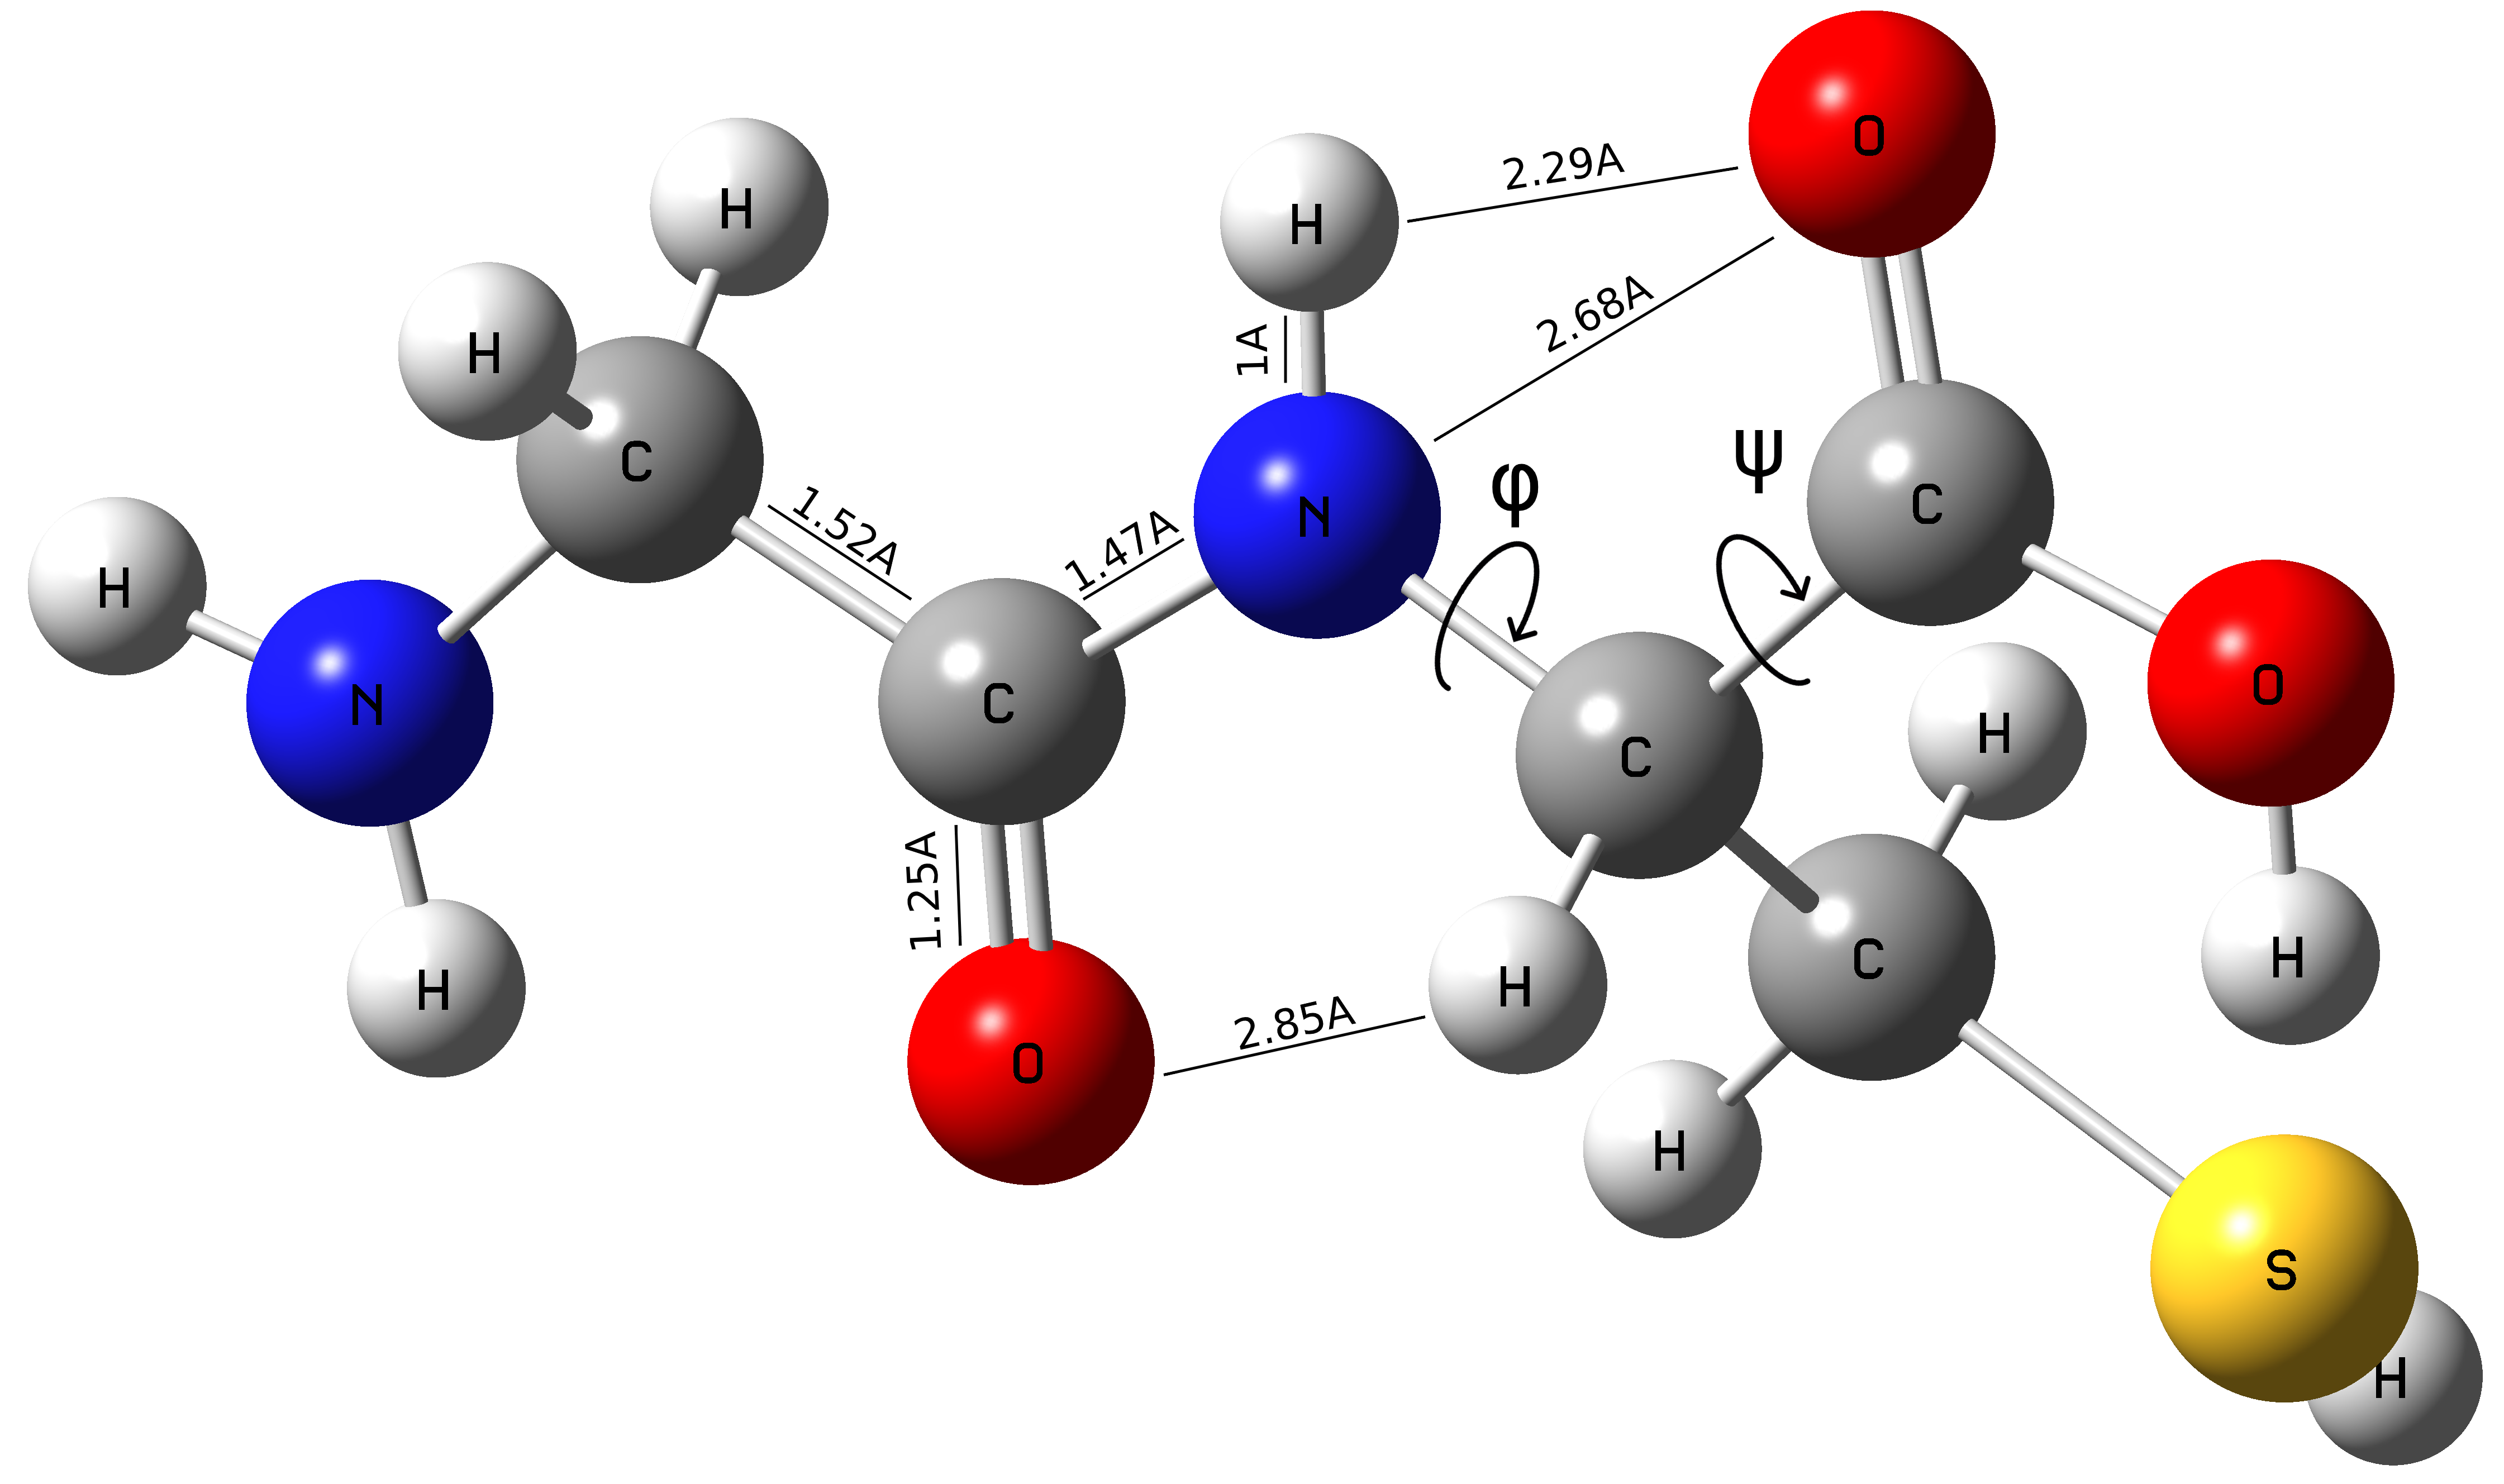
\includegraphics[scale=0.15]{GlyCys3D.png}
        \caption{Dipéptido 3D Ala-Cys.}
    \end{figure}
    % END FIGURE %

    % START FIGURE %
    \begin{figure}[h!]
        \centering
        \begin{minipage}[b]{0.49\textwidth}
            \centering
          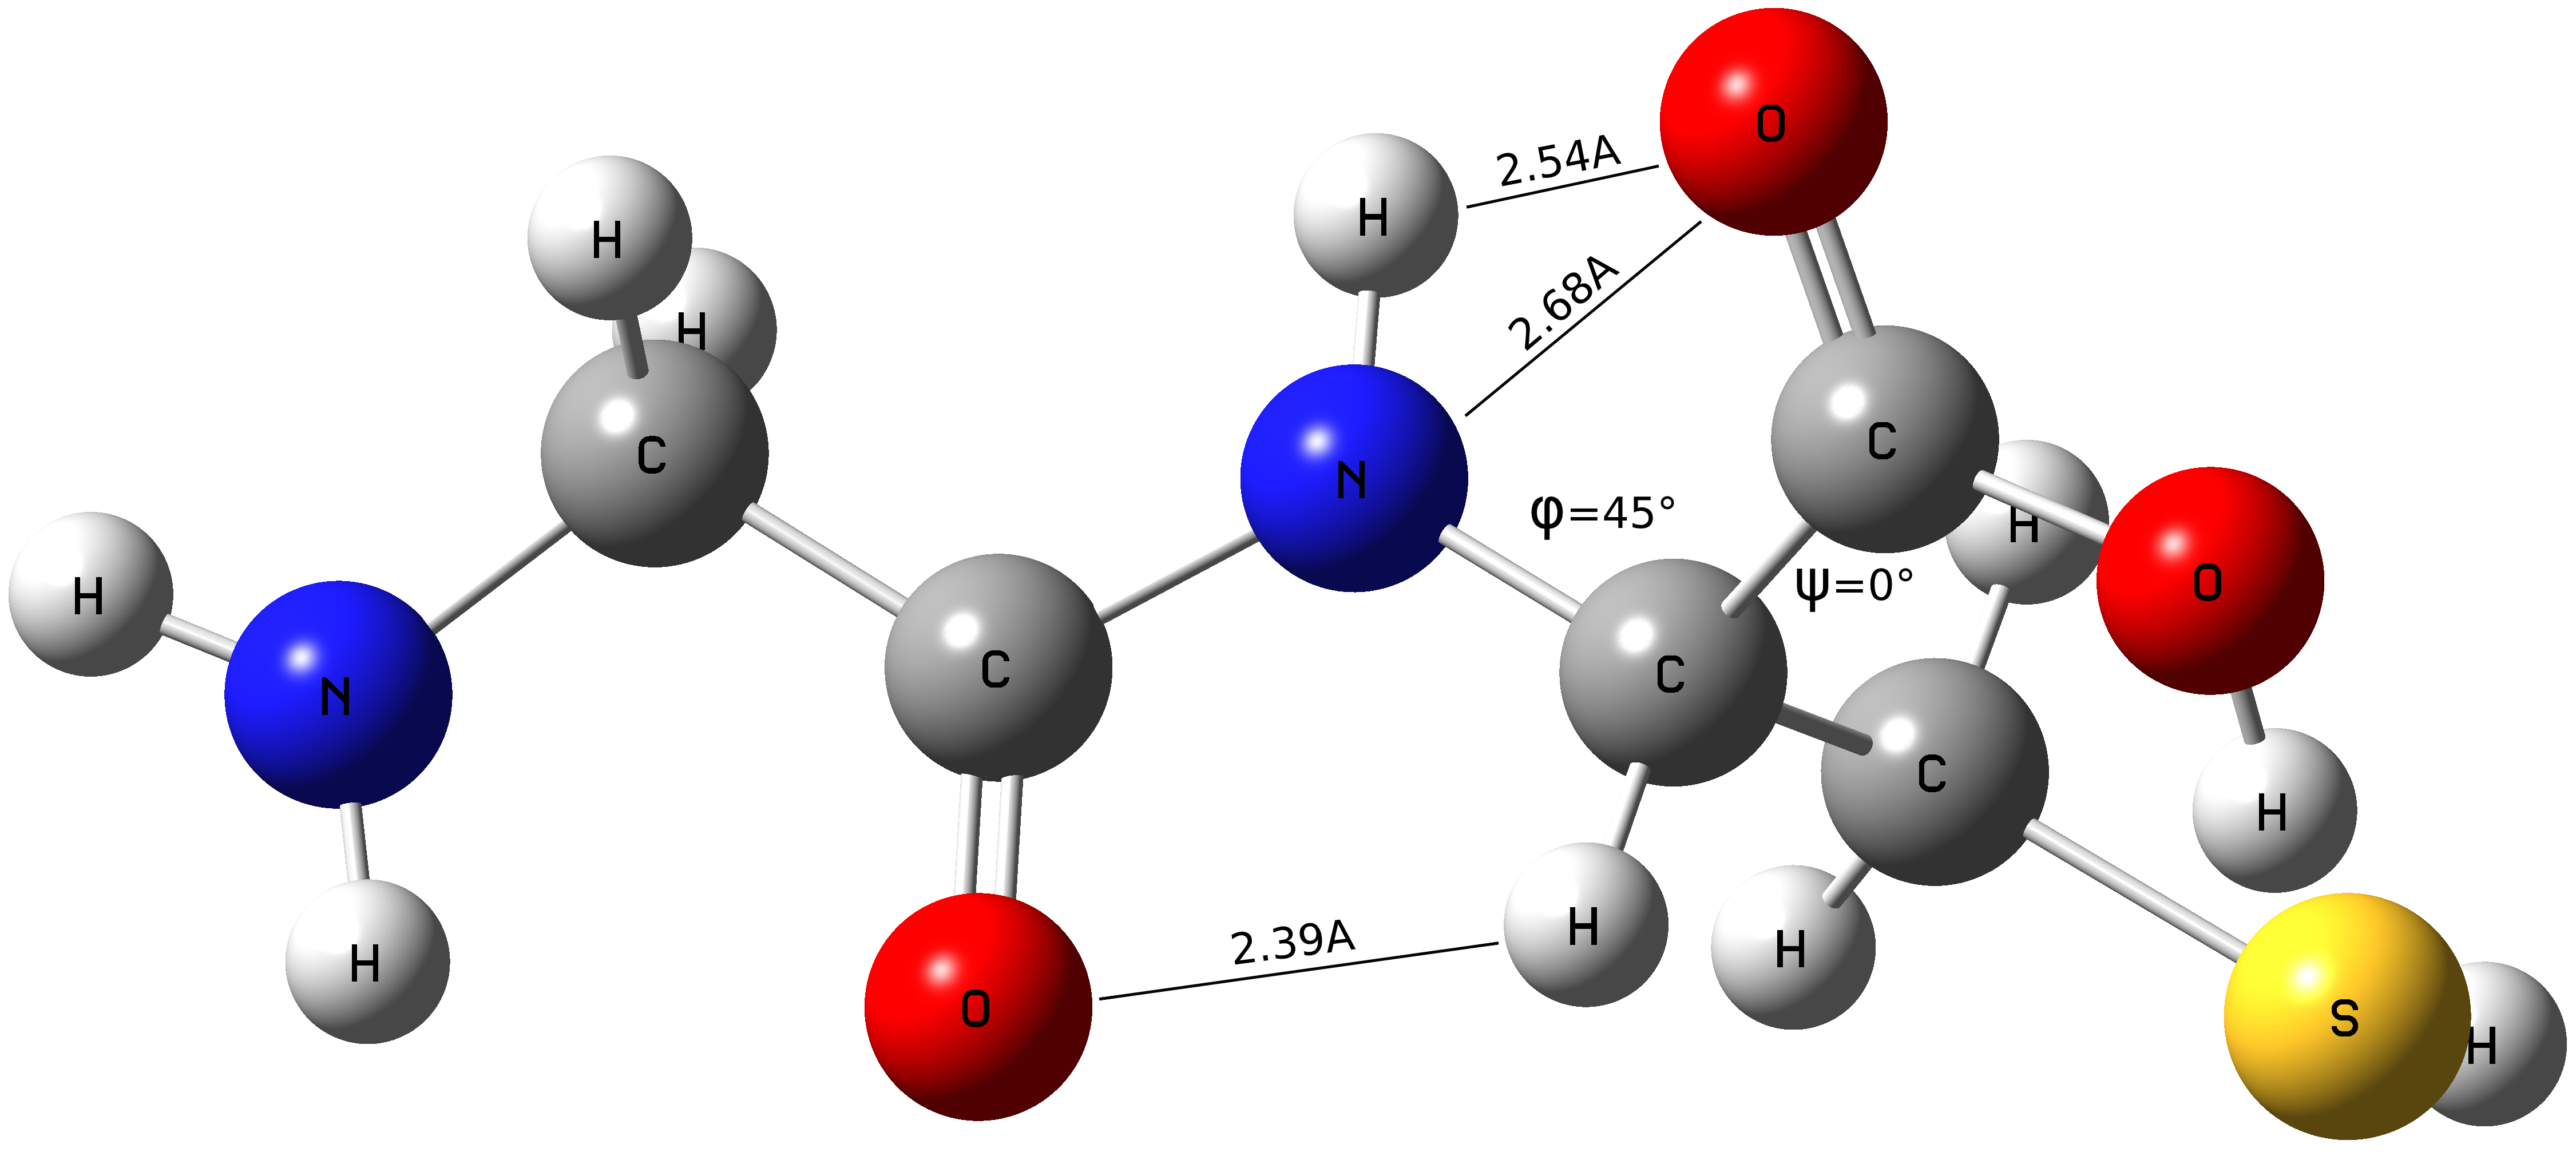
\includegraphics[scale=0.085]{GlyCys3D45fi.png}
          \caption{$\phi=45^o$ y $\psi=0^o$}
        \end{minipage}
        \hfill
        \begin{minipage}[b]{0.49\textwidth}
          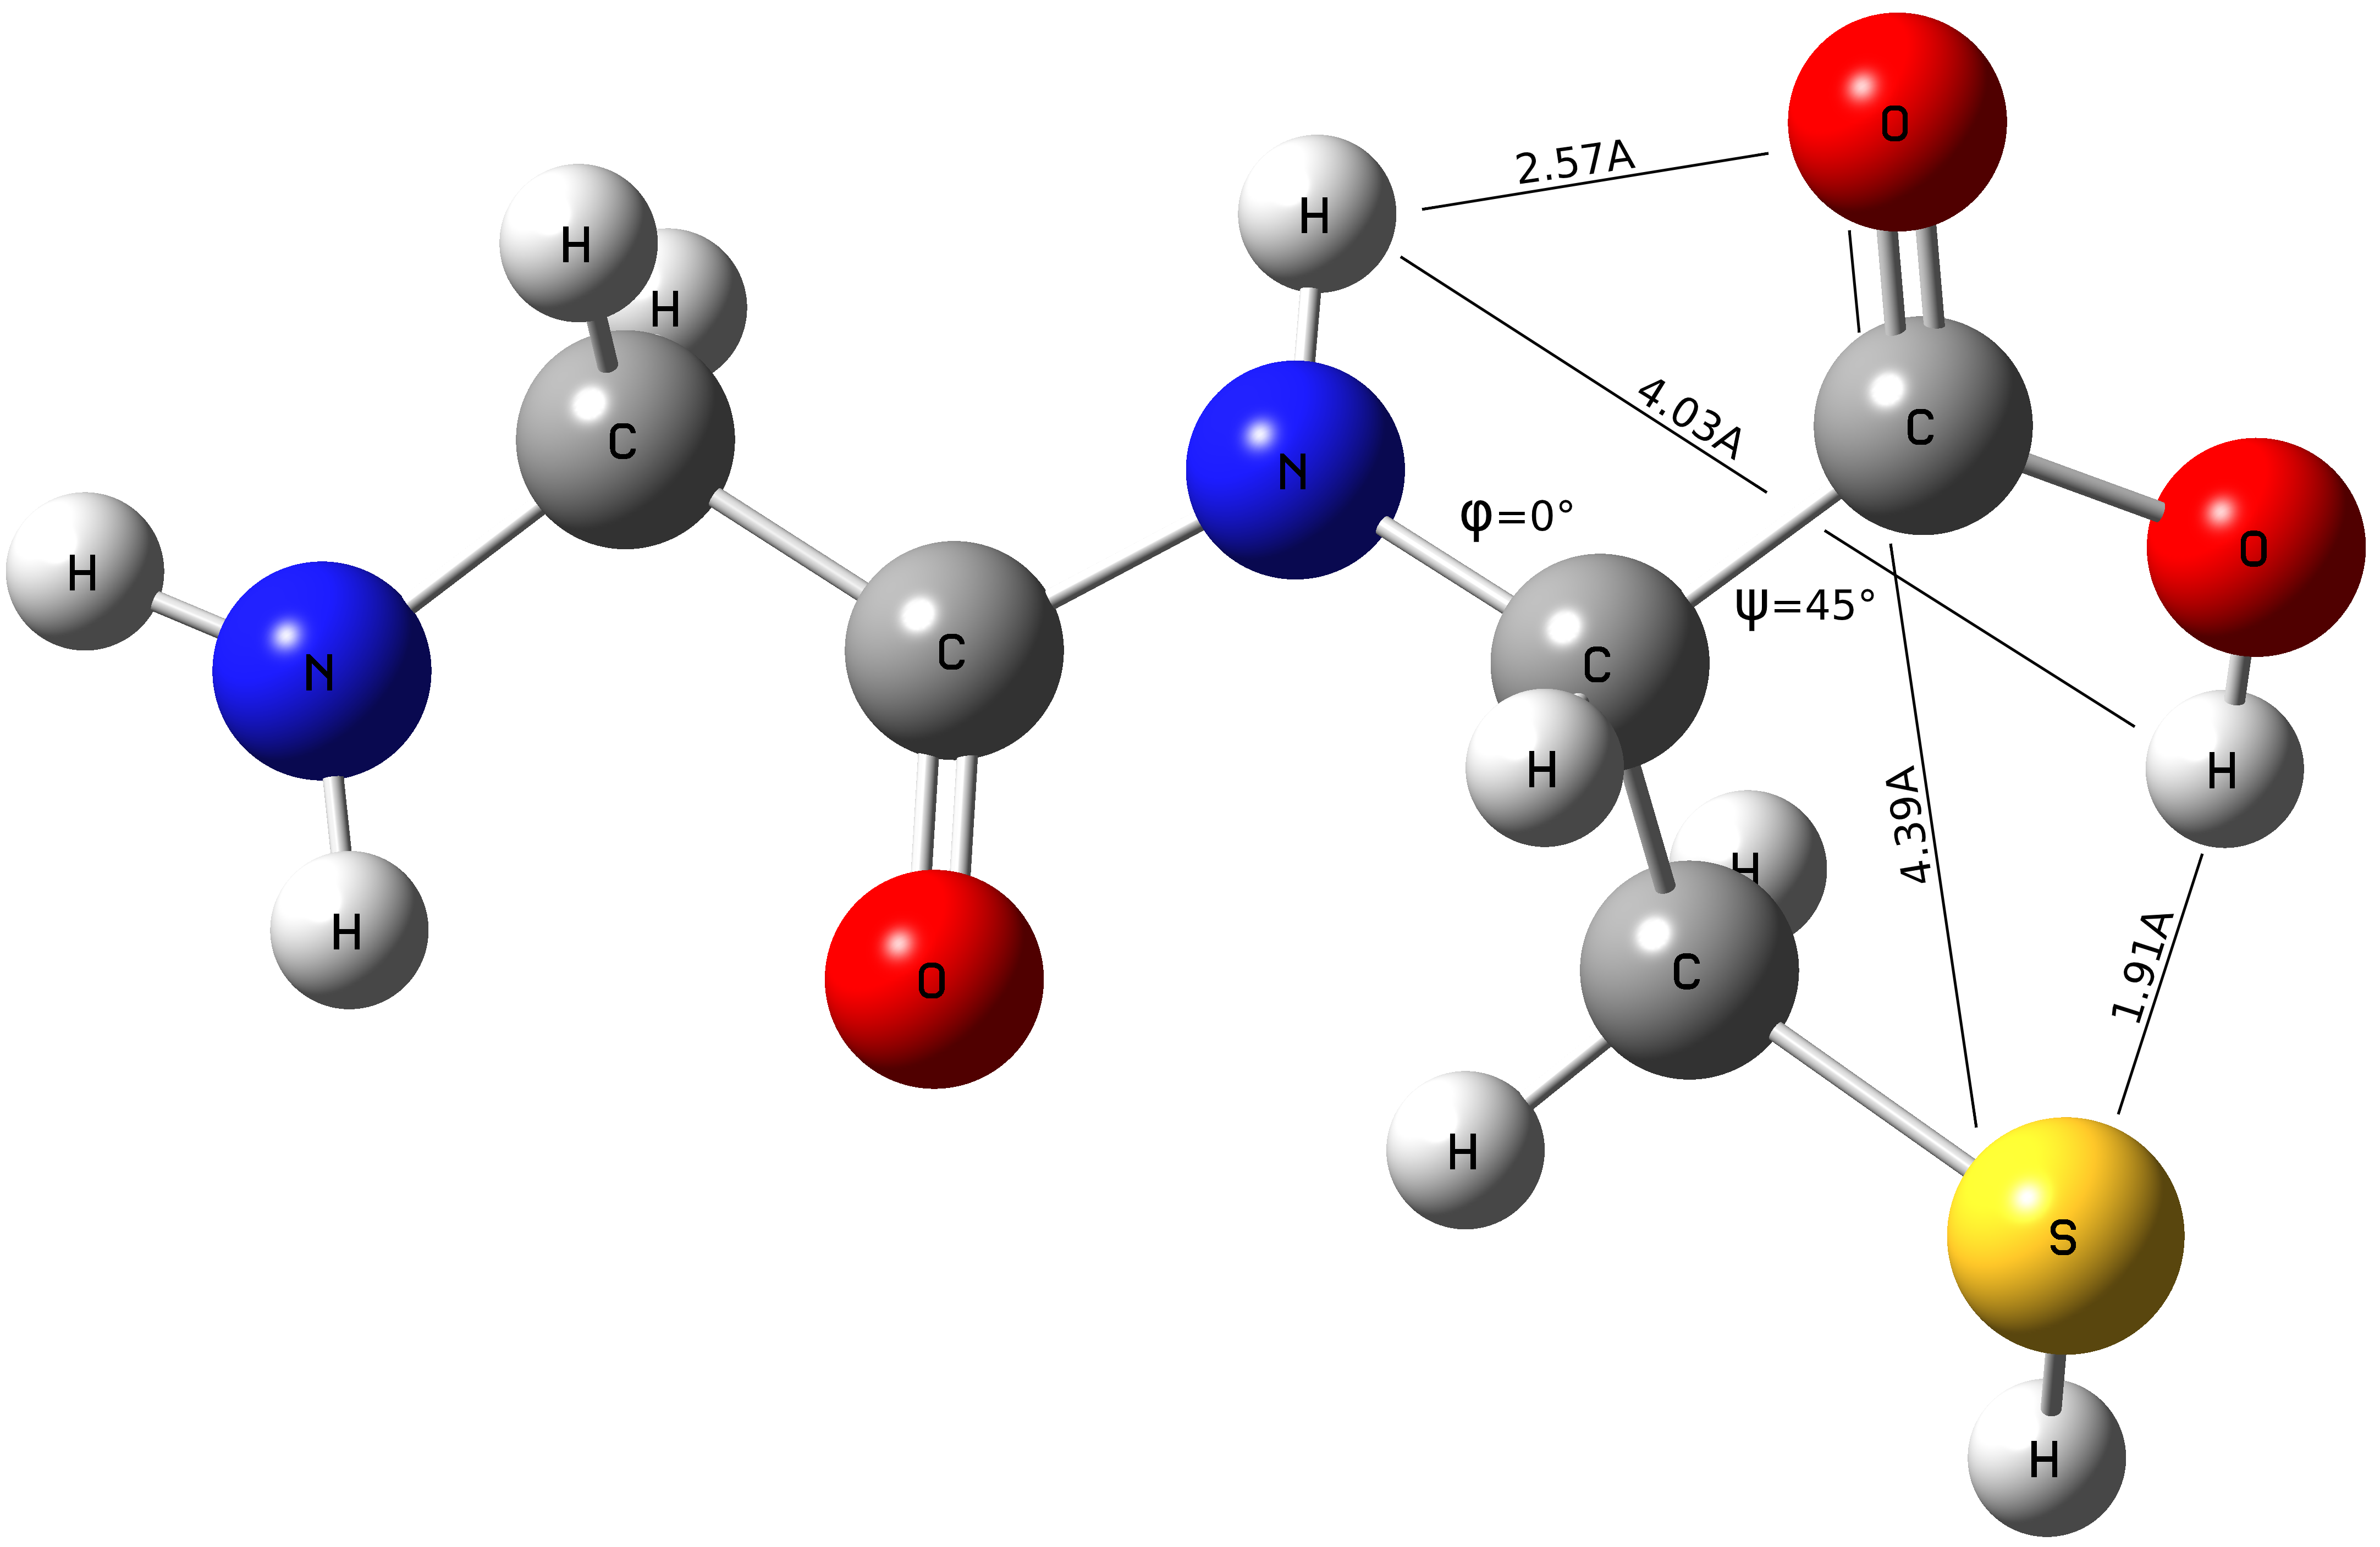
\includegraphics[scale=0.085]{GlyCys3D45psi.png}
          \caption{$\phi=0^o$ y $\psi=45^o$}
        \end{minipage}
        \begin{minipage}[b]{0.49\textwidth}
            \centering
          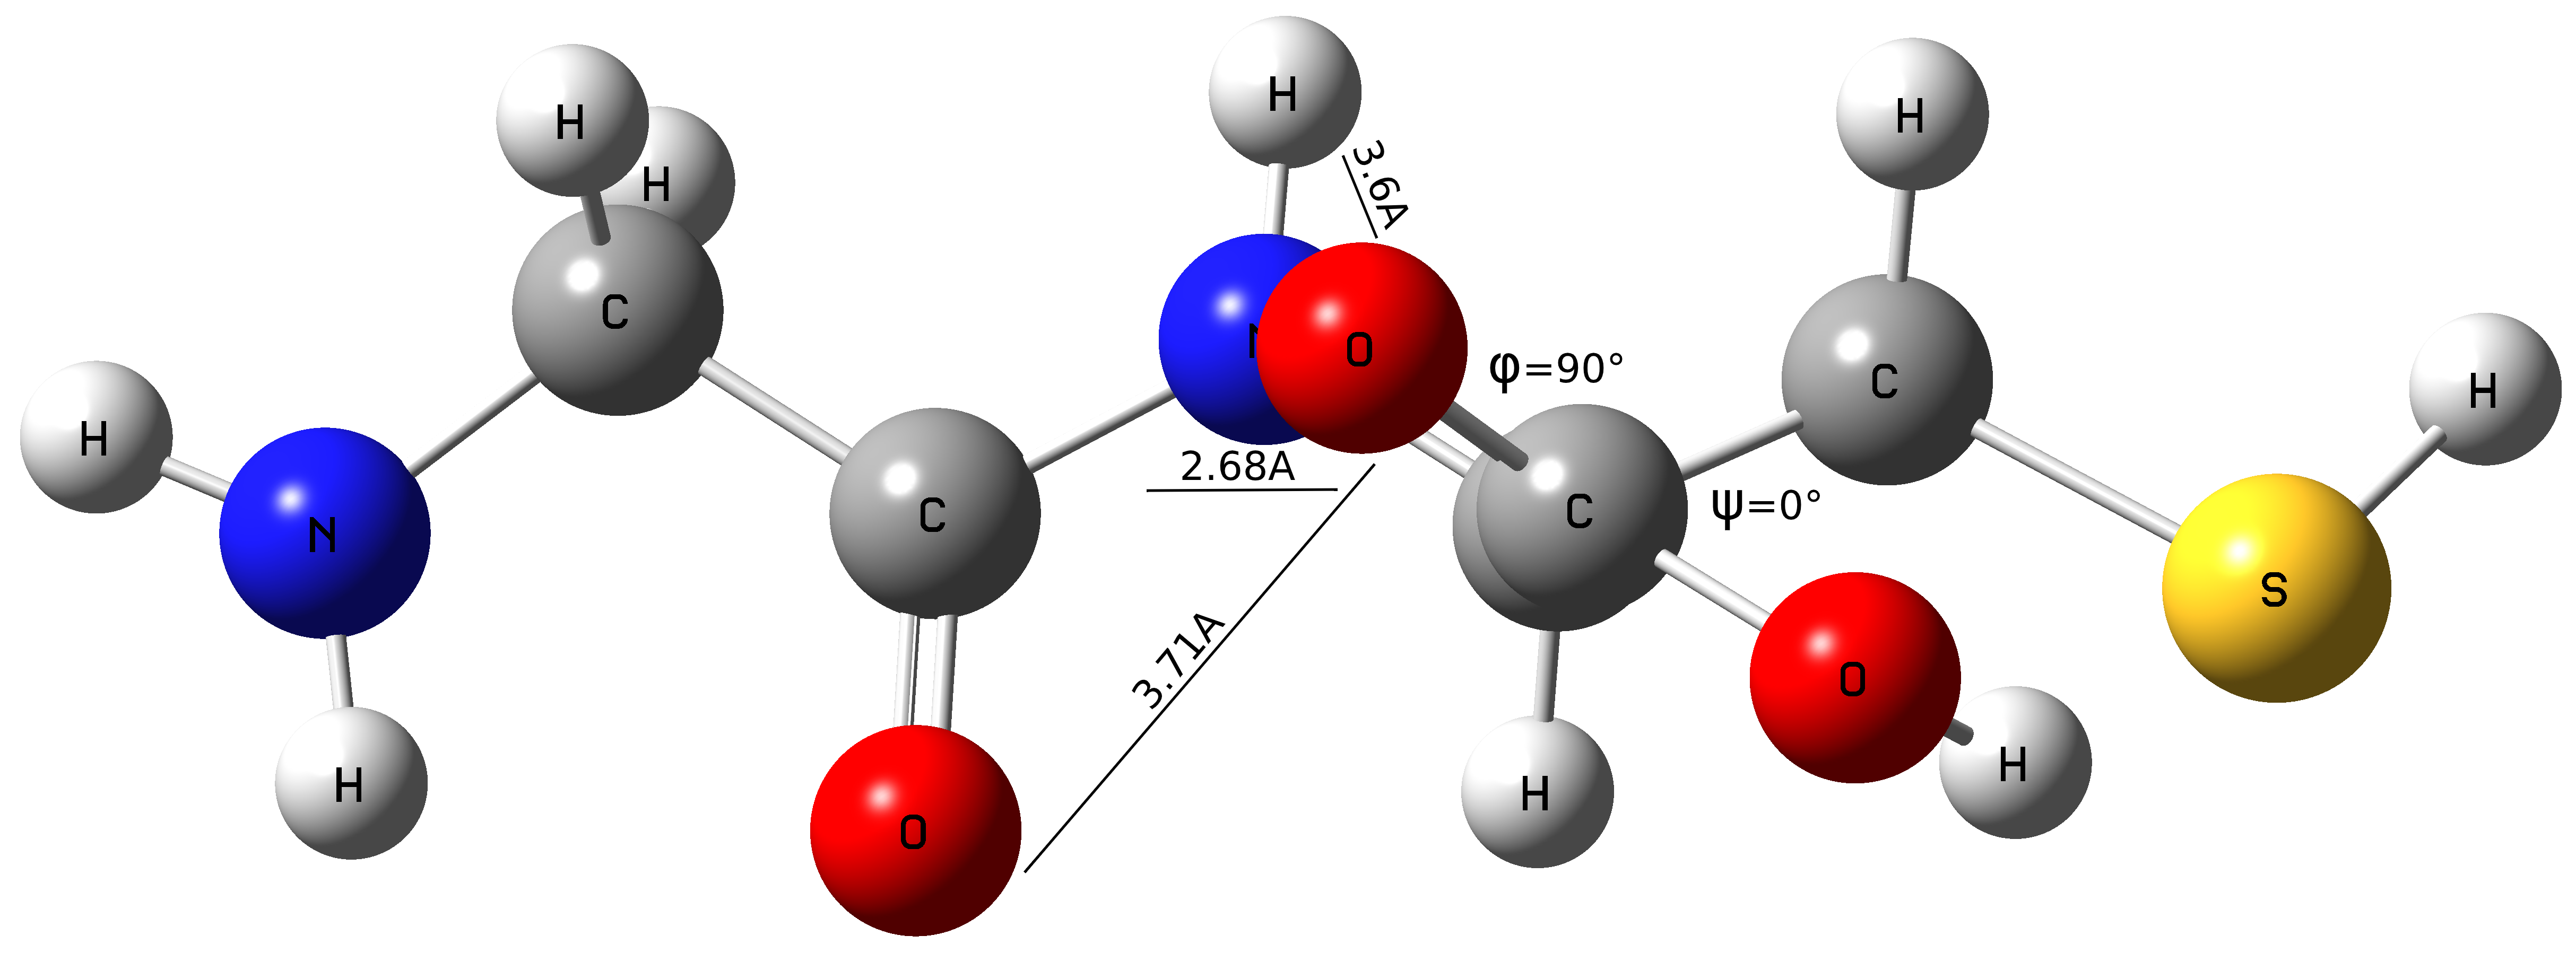
\includegraphics[scale=0.085]{GlyCys3D90fi.png}
          \caption{$\phi=90^o$ y $\psi=0^o$}
        \end{minipage}
        \hfill
        \begin{minipage}[b]{0.49\textwidth}
          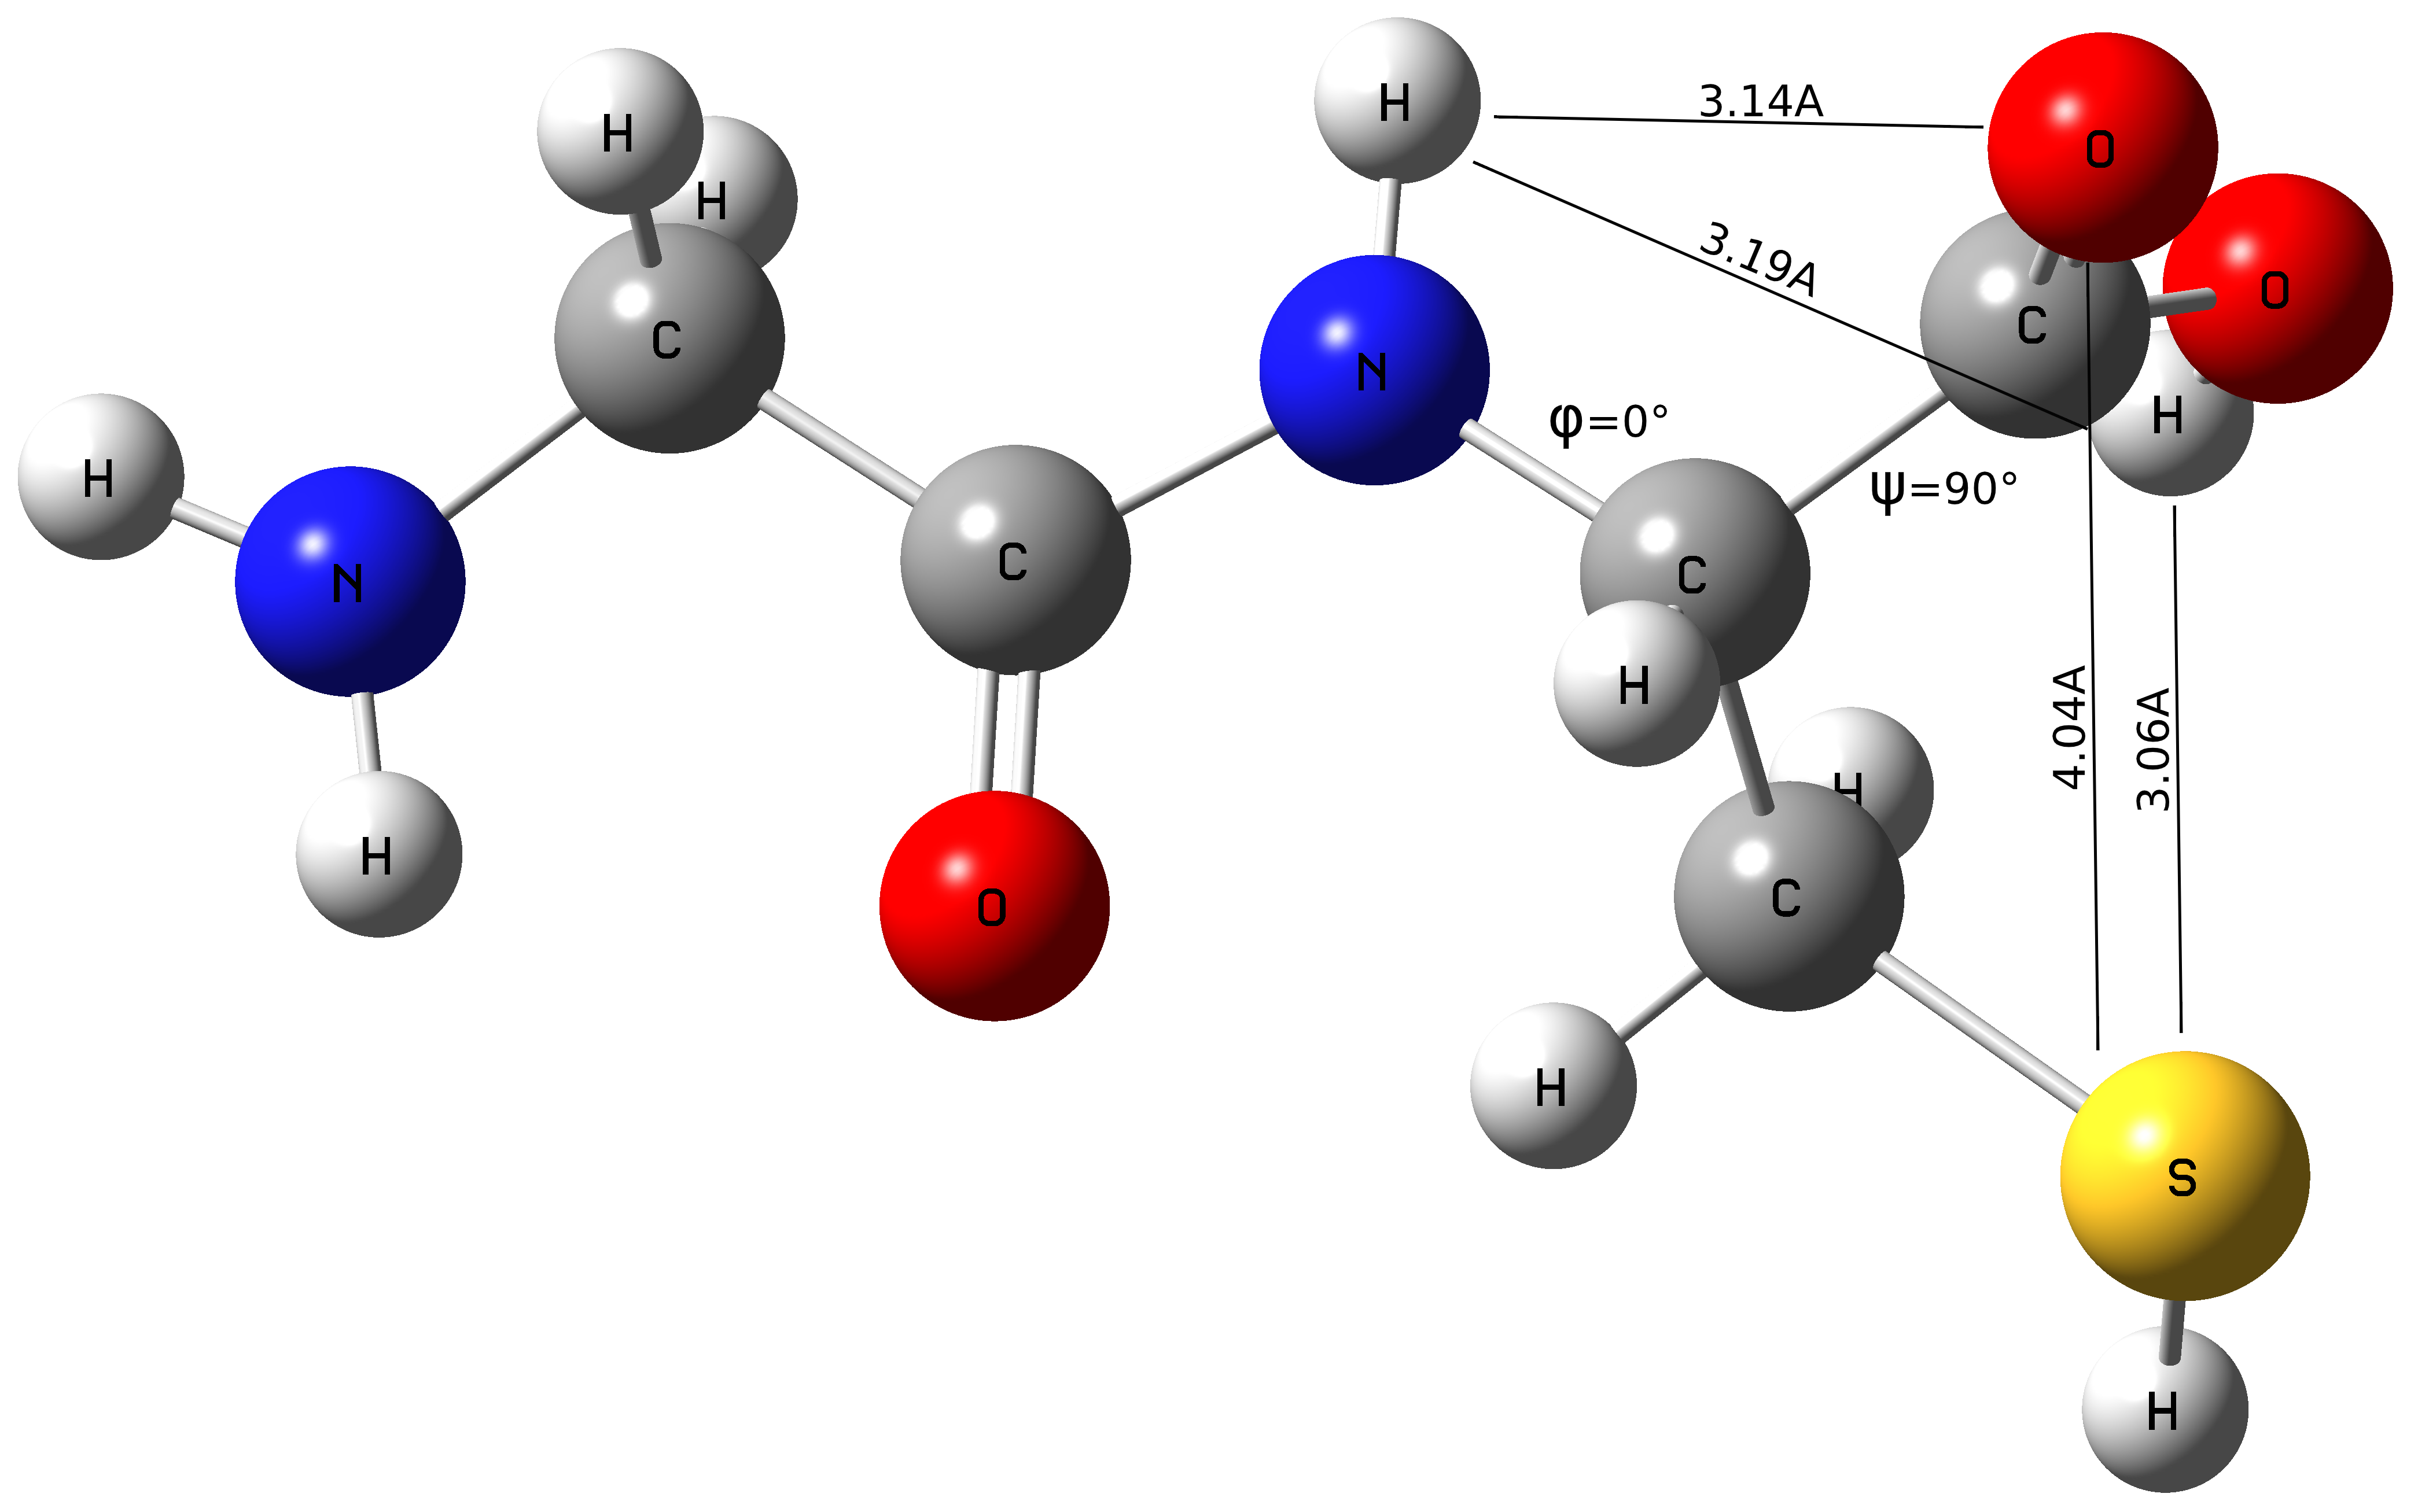
\includegraphics[scale=0.085]{GlyCys3D90psi.png}
          \caption{$\phi=0^o$ y $\psi=90^o$}
        \end{minipage}
        \begin{minipage}[b]{0.49\textwidth}
            \centering
          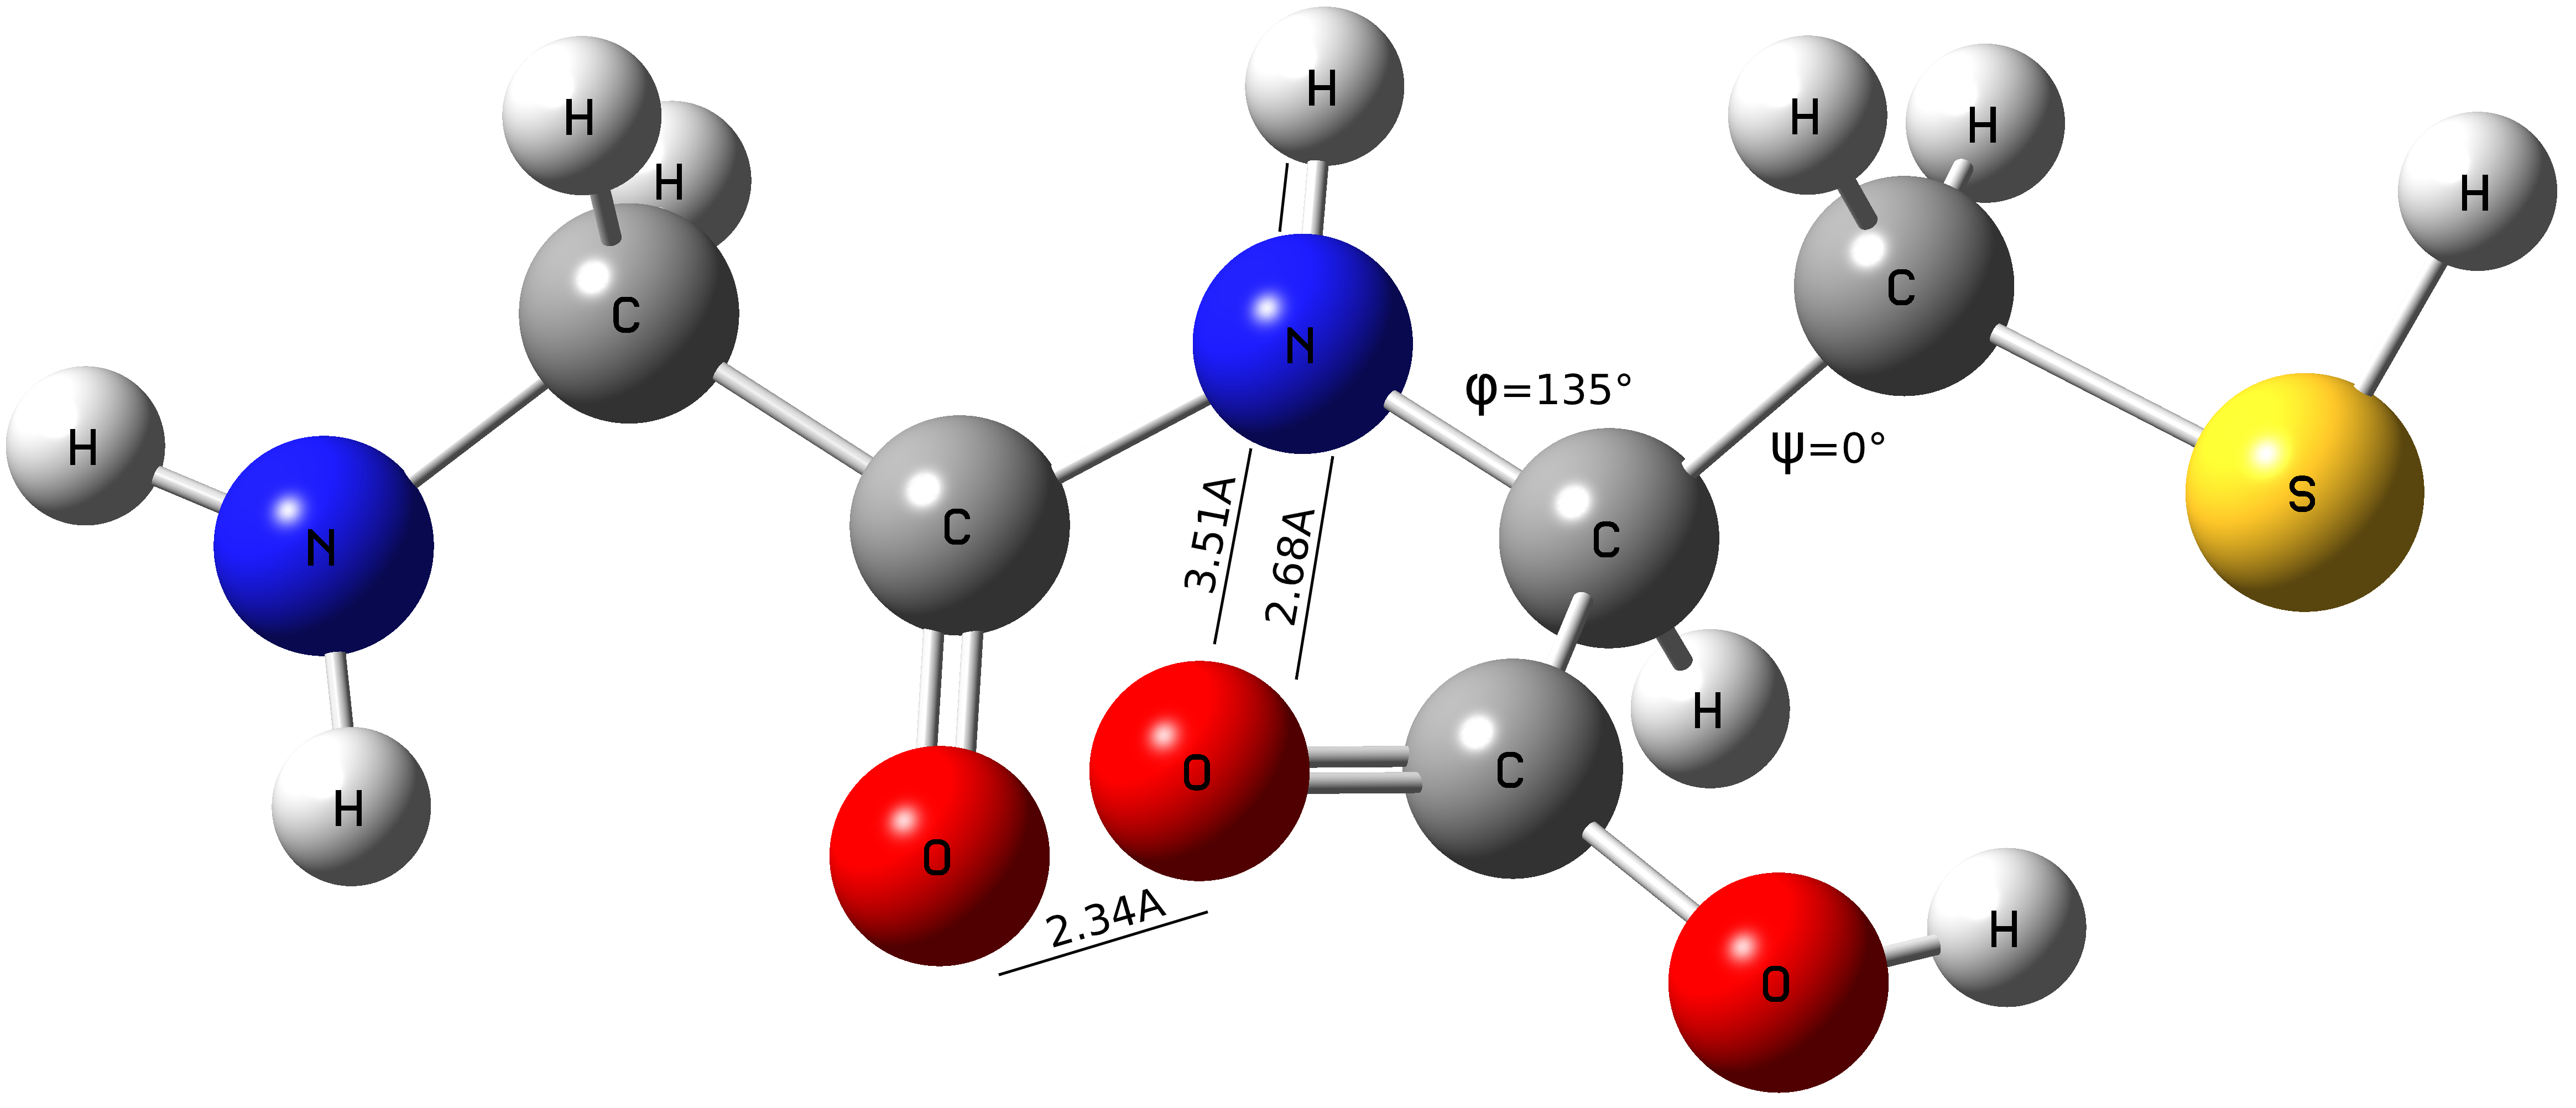
\includegraphics[scale=0.085]{GlyCys3D9135fi.png}
          \caption{$\phi=135^o$ y $\psi=0^o$}
        \end{minipage}
        \hfill
        \begin{minipage}[b]{0.49\textwidth}
          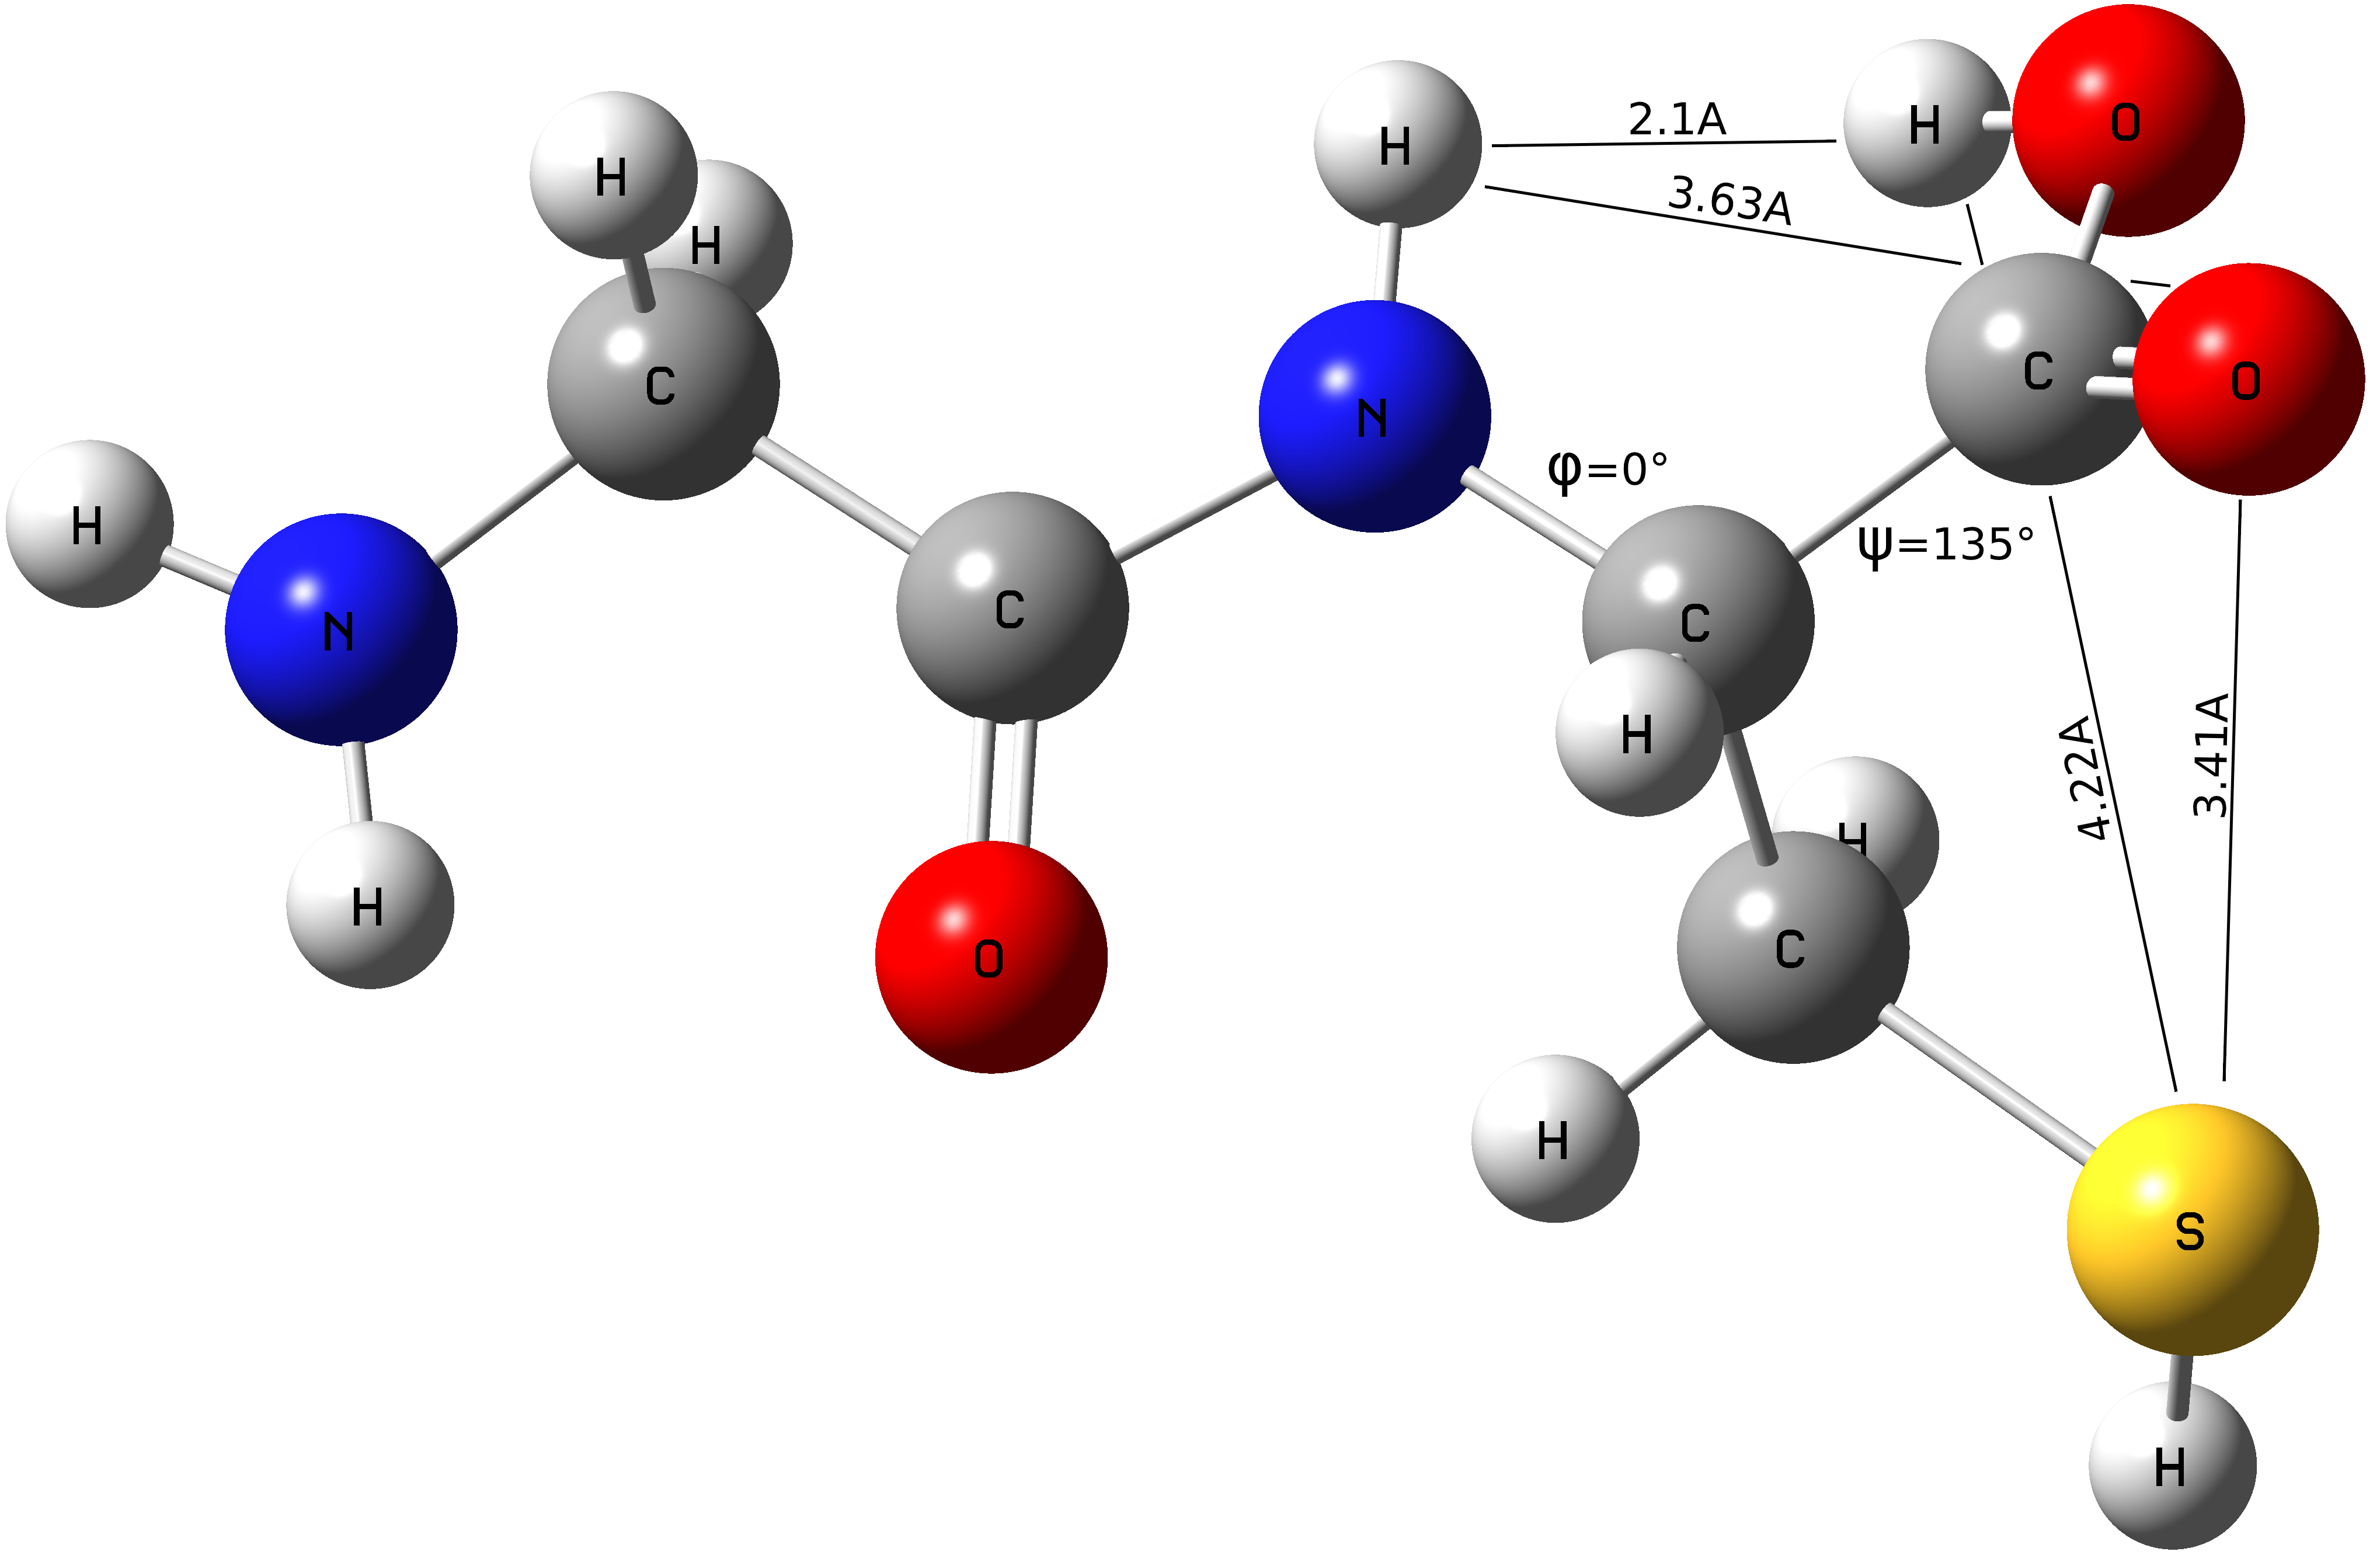
\includegraphics[scale=0.085]{GlyCys3D135psi.png}
          \caption{$\phi=0^o$ y $\psi=135^o$}
        \end{minipage}
        \begin{minipage}[b]{0.49\textwidth}
            \centering
          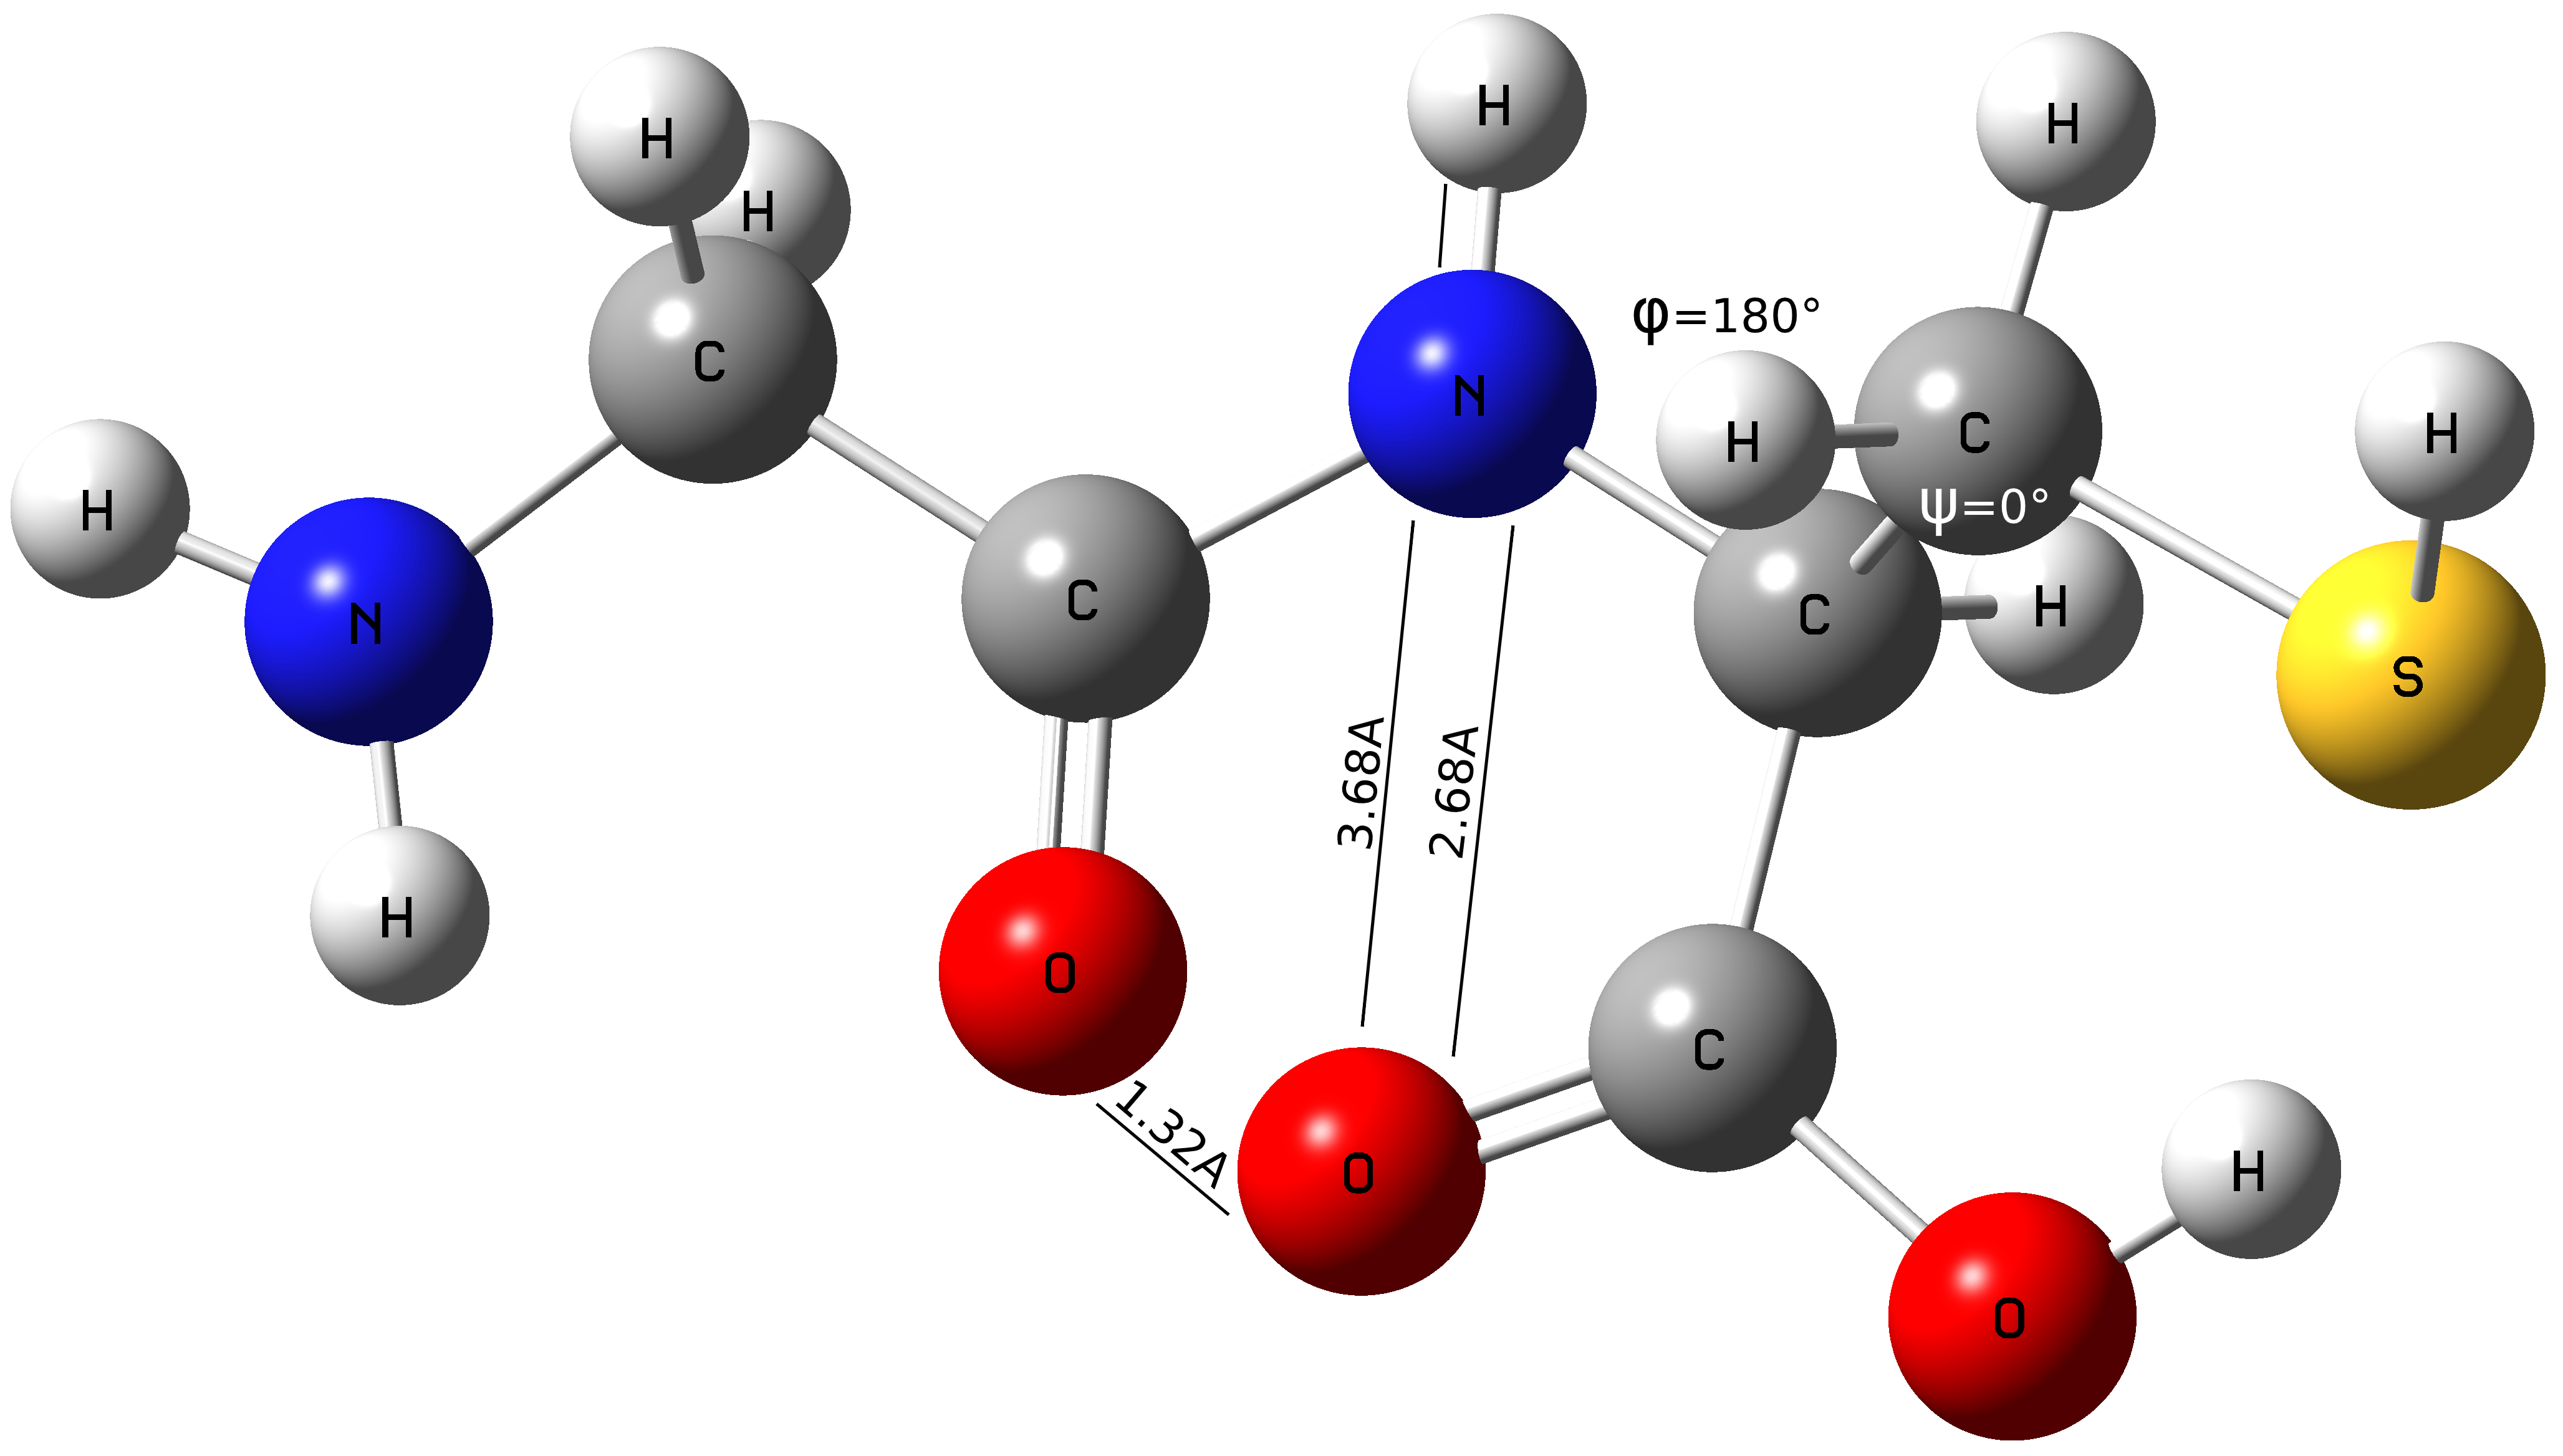
\includegraphics[scale=0.085]{GlyCys3D9180fi.png}
          \caption{$\phi=180^o$ y $\psi=0^o$}
        \end{minipage}
        \hfill
        \begin{minipage}[b]{0.49\textwidth}
          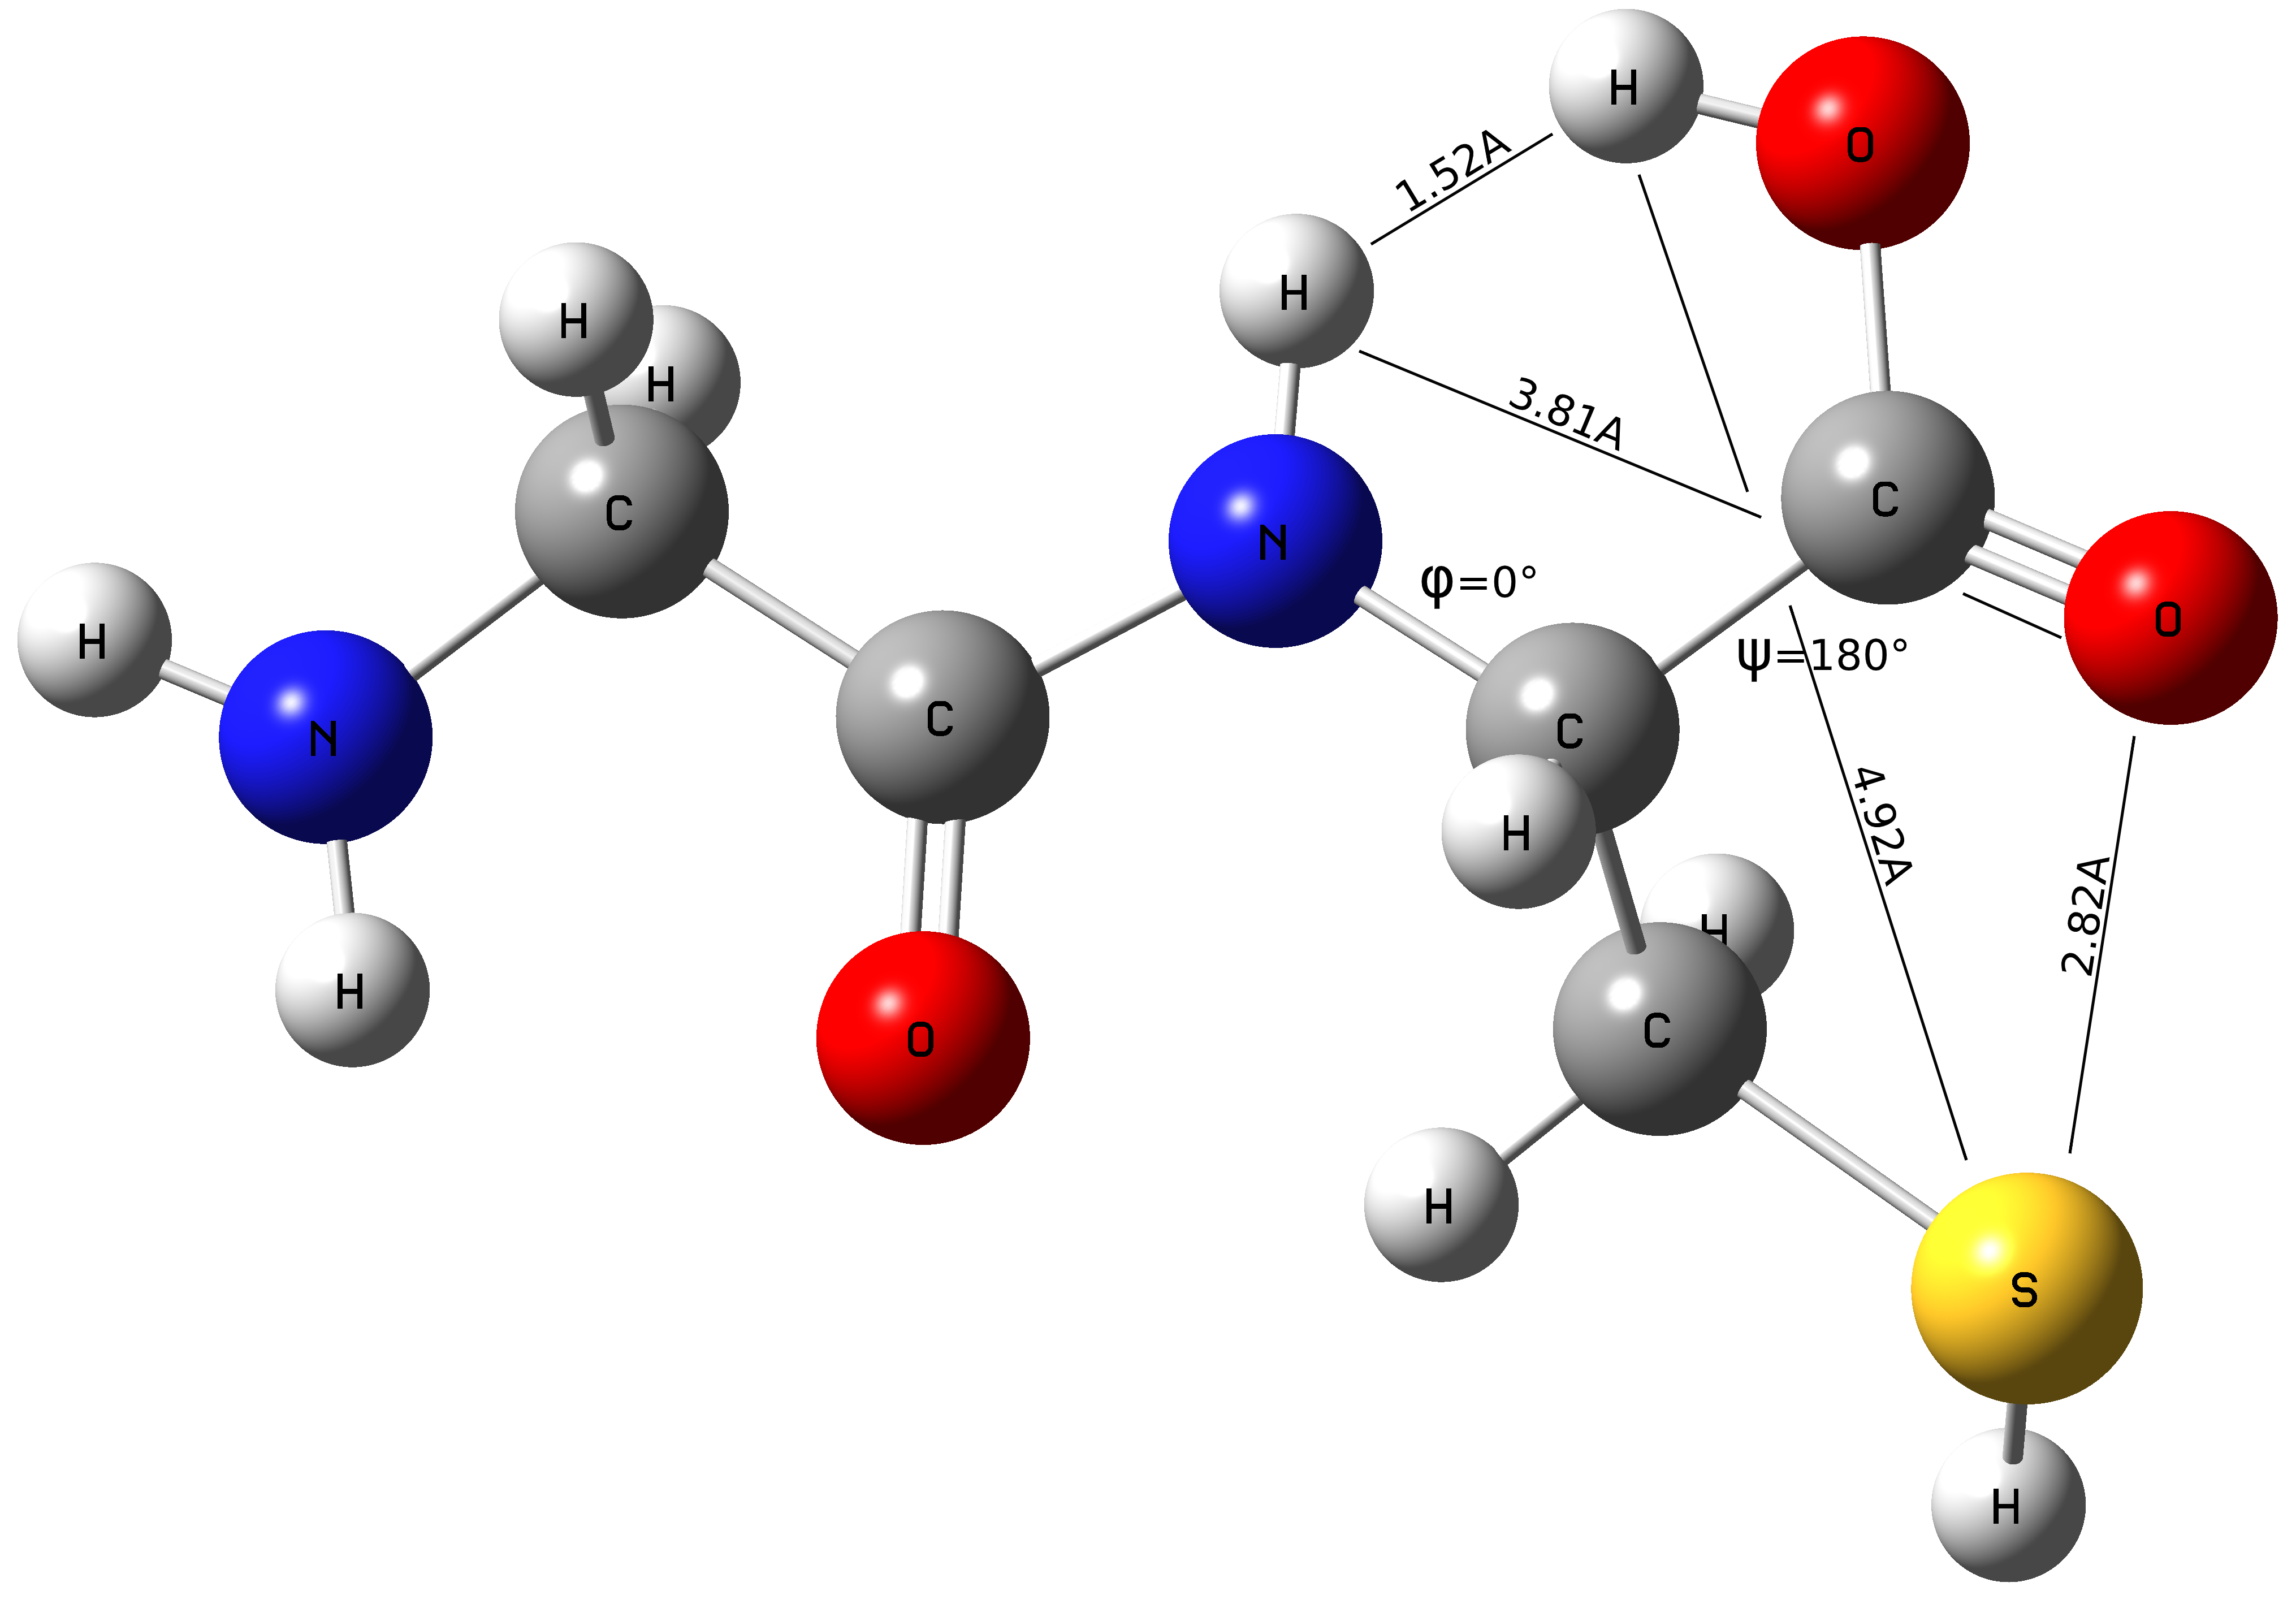
\includegraphics[scale=0.085]{GlyCys3D180psi.png}
          \caption{$\phi=0^o$ y $\psi=180^o$}
        \end{minipage}
    \end{figure}
    % END FIGURE %

    % START FIGURE %
    \begin{figure}[h]
        \centering
        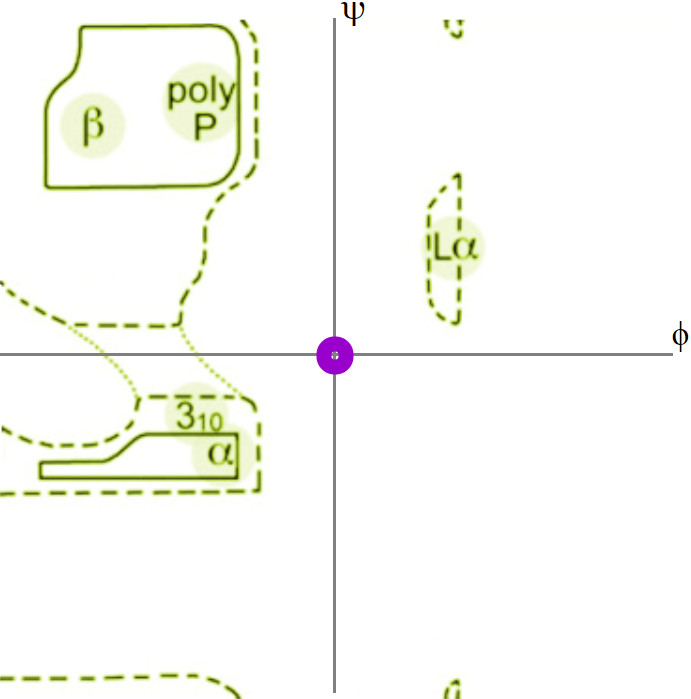
\includegraphics[scale=0.35]{diagrama.jpg}
        \caption{Diagrama de Ramachandran.}
    \end{figure}
    % END FIGURE %

    \np{Los ángulos diedros $\phi$ y $\psi$ del dipéptido formado se muestran en la figura 2 y en las siguientes figuras se muestran los ángulos dihedricos probados.}

    \np{Al comparar los ángulos $\phi$ y $\psi$ realizados con la figura, se puede apreciar los ángulos $\phi$ y $\psi$ que están sobre los ejes positivos, que van de $0-180^o$ no presentan alguna estructura secundaria.}

    \np{Además de esto al comparar las distancias de enlace entre los átomos a diferentes valores de $\phi$ y $\psi$, se puede observar hay ángulos que no están permitidos debido a que la distancia de enlace las cuales se ven reducidas, lo cual corrobora que las estructuras secundarias solo pueden formarce en ciertos valores $\phi$ y $\psi$ donde no se presente el impedimento estérico.}


    
    %PROBLEMA 7%
    
    \np{\bt{7)}Construya ahora un péptido con 12 residuos de aminoácido y acomódelo de forma que obtenga una conformación totalmente extendida.¿Cuáles son los valores de los ángulos de torsión $\phi$ y $\psi$? Compare su polipéptido con alguna imagen de hojas betas que haya en algún libro. ¿Es esta conformación es la que se observa en las hojas beta? Ahora haga un giro beta entre el residuo 6 y 7 para formar una hoja beta ¿Hacia adonde apuntan las cadenas laterales o grupos R? ¿Cuál es la distancia de los puentes de hidrógeno? ¿Poseen la misma distancia?}   
    

    % START FIGURE %
    \begin{figure}[h!]
        \centering
        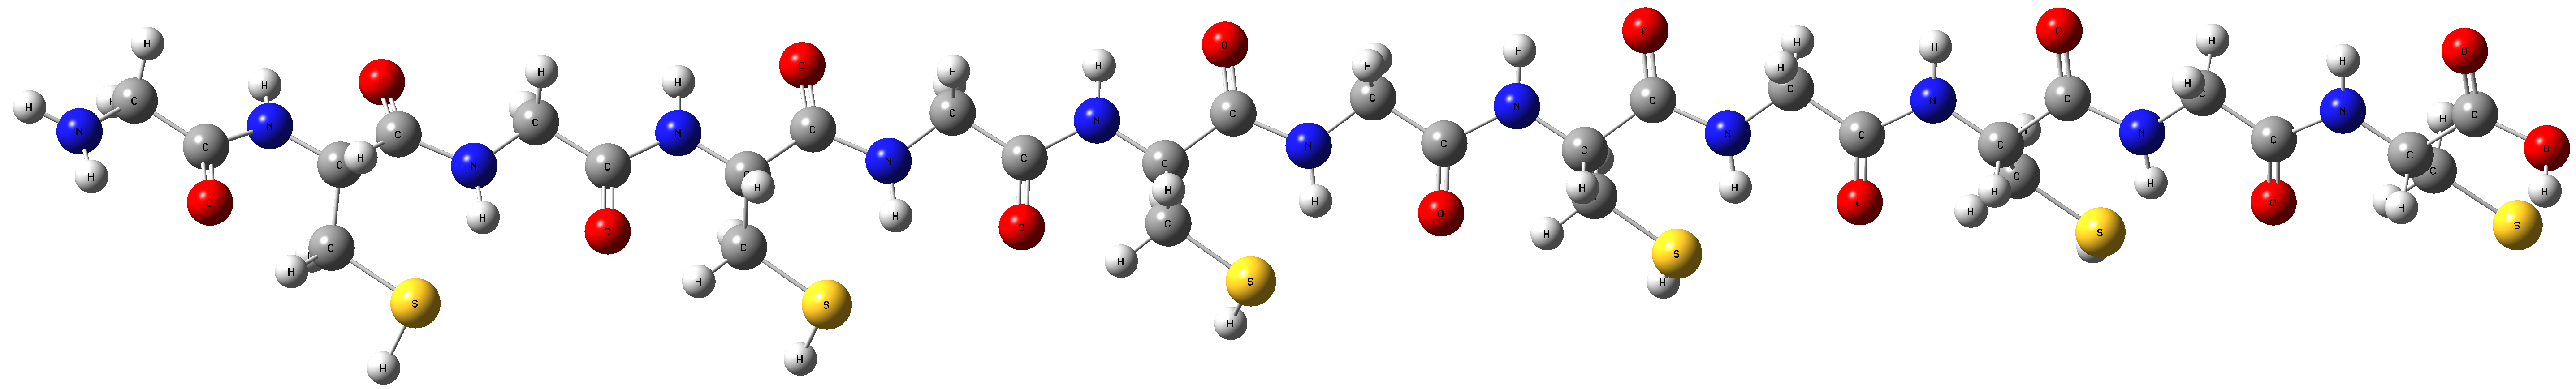
\includegraphics[scale=0.15]{12pep.png}
        \caption{6(Gly-Cys)}
    \end{figure}
    % END FIGURE %

    % START FIGURE %
    \begin{figure}[h!]
        \centering
        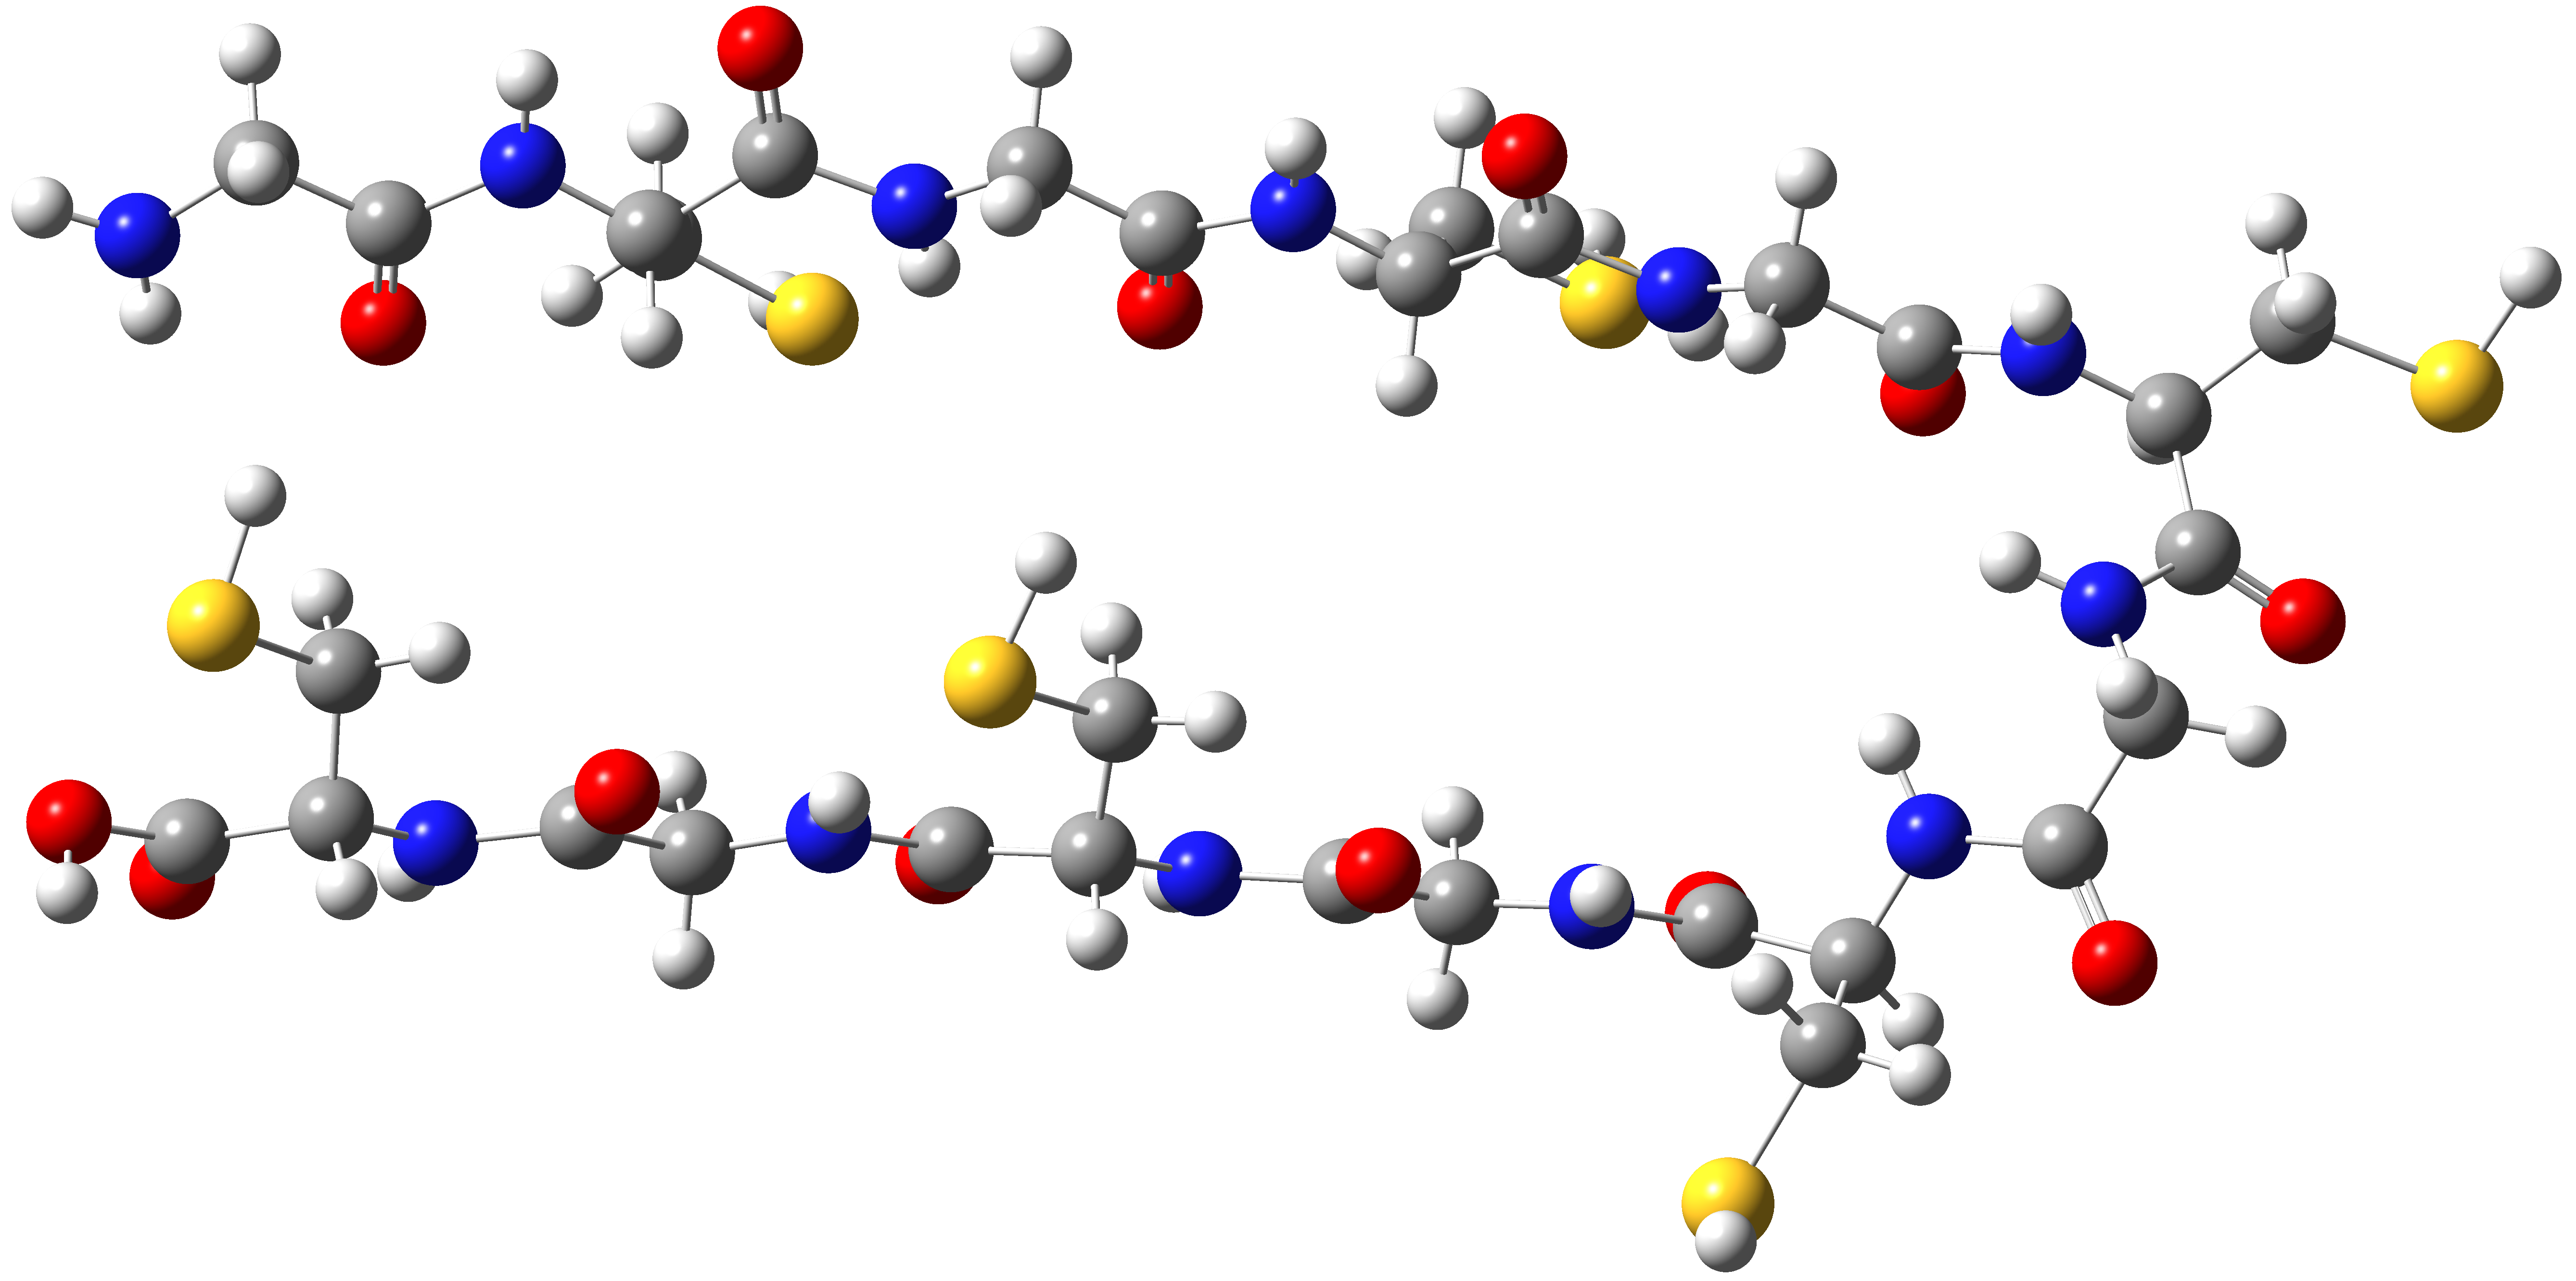
\includegraphics[scale=0.12]{hojab.png}
        \caption{Hoja beta}
    \end{figure}
    % END FIGURE %

    \np{Los ángulos $\phi$ y $\psi$ valen cero en toda la cadena peptidica, la conformación observada no es de una hoja beta, además de que los valores de $\phi$ y $\psi$ no corresponden a los de una hoja beta como se muestra en el gráfico de Ramachandran.}

    \np{Las cadenas laterales estan apuntando hacia arriba y abajo de los planos peptídicos, la distancia no la pude medir por que no logre orientar la hoja beta, al estudiar la estructura de la hoja beta se puede esperar que las distancias sean iguales o muy parecidas entre si.}

    \np{NOTA: No me supe como realizar la hoja b de forma adecuada y el alfa hélice, trate de hacer la hoja beta pero al realizarla no supe como rotar los ángulos $\phi$ y $\psi$ del carbono alfa en el giro, por lo que los puentes de hidrógeno no quedan orientados como deberían para mantener la estructura hoja beta, si me pudiera orientar para poder realizarla de forma correcta se lo agradeceria.}
    
    \np{\bt{8)} ¿Cuáles son esos valores de $\phi$ y $\psi$ que debe tener un péptido para formar una alfa helice?} 


    \np{Al observar el gráfica de Ramachandran se pueda apreciar que las alfa helices se encuentran en el tercer cuadrande con valores $\phi$ y $\psi$.}

    %PROBLEMA 9%

    \np{\bt{9)} Cual de los siguientes tripéptidos será mas soluble en una disolución 1M de NaOH}
    % START FIGURE %
    \begin{figure}[h!]
        \centering
        \begin{minipage}[b]{0.49\textwidth}
            \centering
          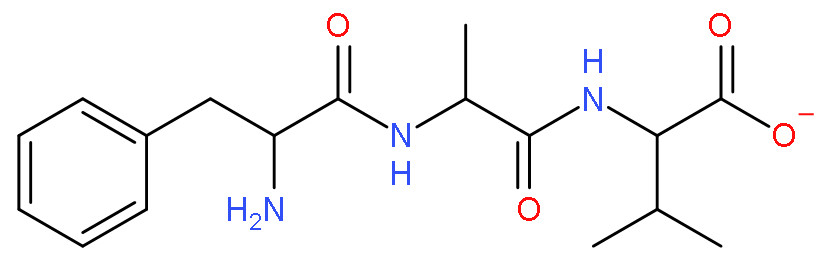
\includegraphics[scale=0.4]{PheAlaVal.jpg}
          \caption{Phe-Ala-Val.}
        \end{minipage}
        \hfill
        \begin{minipage}[b]{0.49\textwidth}
          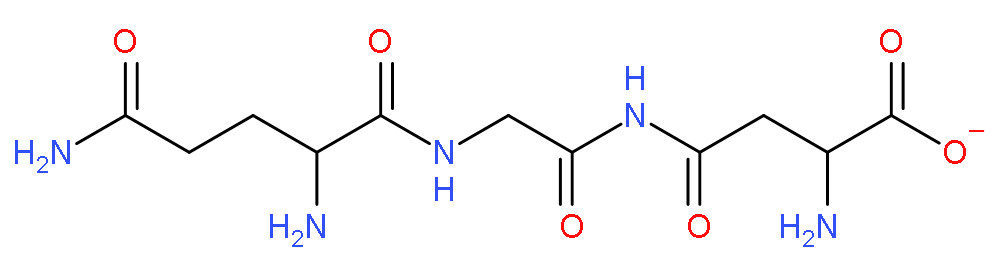
\includegraphics[scale=0.4]{GlnGlyAsn.jpg}
          \caption{Gln-Gly-Asn.}
        \end{minipage}
        \hfill
        \begin{minipage}[b]{0.49\textwidth}
            \centering
          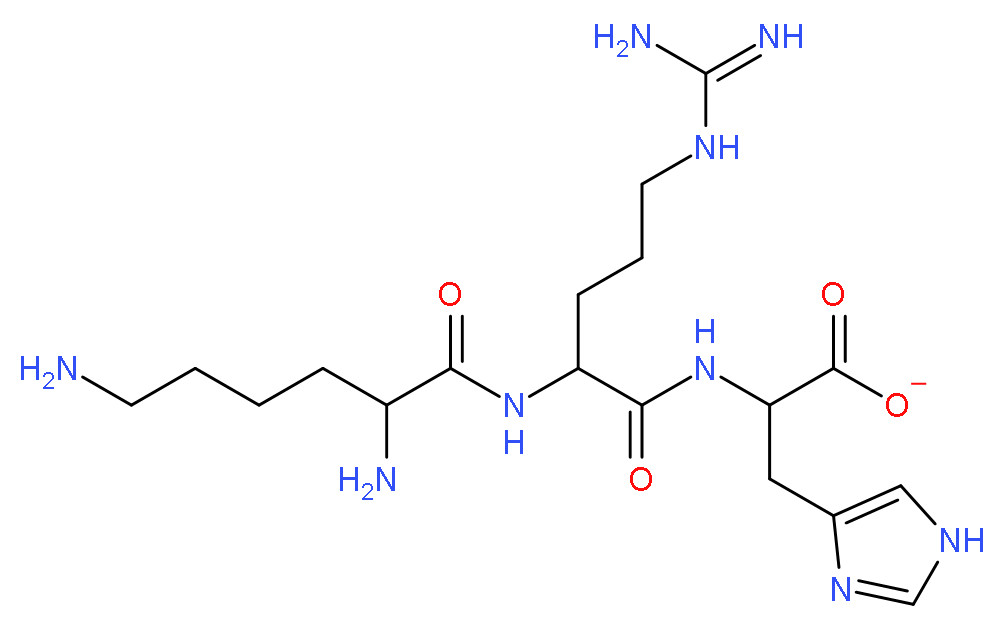
\includegraphics[scale=0.40]{LysArgHis.jpg}
          \caption{Lys-Arg-His.}
        \end{minipage}
        \hfill
        \begin{minipage}[b]{0.49\textwidth}
          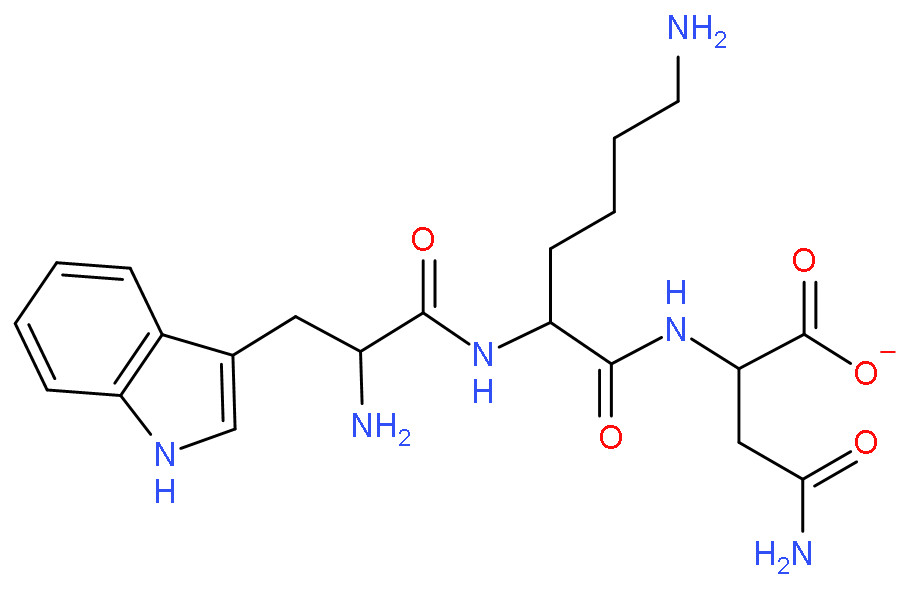
\includegraphics[scale=0.40]{TrpLysAsp.jpg}
          \caption{Trp-Lys-Asp.}
        \end{minipage}
        \hfill
        \begin{minipage}[b]{0.95\textwidth}
            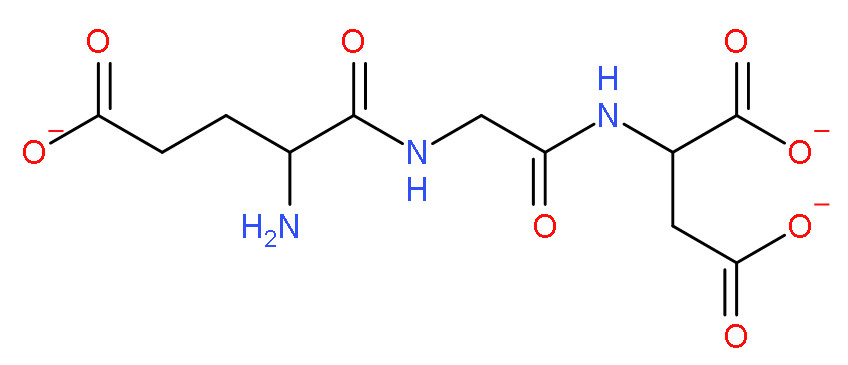
\includegraphics[scale=0.45]{GluGlyAsp.jpg}
            \caption{Glu-Gly-Asn.}
          \end{minipage}
    \end{figure}
    % END FIGURE %
 

    \np{Al construir las estructuras de los tripéptidos en un médio básico, se observa que el tripéptido Glu-Gly-Asn posse tres cargas, por lo que tendrá más intreacciones ion-dipolo con el disolvente, lo cual es energéticamente favorable, por lo que será más soluble que los demás tripéptidos.} 
    
    \np{En el caso de los demás tripétidos, al tener solo una carga negativa, la solubilidad estaría influenciada principalmente con el número de puentes de hidrógeno que es capaz de formar, como en el caso del Lys-Arg-His y Trp-Lys-Asp que pueden forman 8 puentes de hidrógeno por lo que se espera que tengan mayor solubilidad que la Gln-Gly-Asn y Phe-Ala-Val que poseen 7 y 5 respectivamente.}

    %PROBLEMA 10%
    \np{\bt{10)}¿Cuántos pentapéptidos distintos se pueden construir si sólo se emplean aminoácidos polares? ¿Cuántos pentapéptidos distintos se pueden construir si sólo se emplean aminoácidos no polares?}

    \nec{\label{equation:4} \#peptidos=x^n}

    \np{Donde $x$ es el número de aminoácidos que pueden usarse y $n$ es el número de aminoácidos que conforman al péptido.}

    \np{Hay cuatro aminoácidos polares y hay cinco posiciones, usando \eqref{equation:4} se obtiene que:}

    \ec{\#peptidos=(4)^5=~1024~posibles~peptidos}

    \np{Hay ocho aminoácidos no polares y hay cinco posiciones.}

    \ec{\#peptidos=(8)^5=~32,768~posibles~peptidos}

    \end{document}